\section{Thermal profile}
\label{sec:heating}

\begin{keybox}
\begin{itemize}
\item At burnout the air stopped at the tip reaches the stagnation temperature,
\val{A-nominal-T0}--\val{B-nominal-T0}\,\si{\celsius} on a nominal day and
\val{A-hot-T0}--\val{B-hot-T0}\,\si{\celsius} on a hot day. Along the
rest of the nose the air drives the wall towards \val{A-Taw-far-lo}--\val{A-Taw-far-hi}\,K (about
107--110\,\si{\celsius}).
\item The shell is hottest just behind the tip and cools along the nose
(Figure~\ref{fig:thprofile}). The \textbf{outer face} stays below the \SI{120}{\celsius} of the DP490
bond everywhere: at most \val{th-B-nominal-Tout-hi}\,\si{\celsius} on a nominal day, but
\val{th-B-hot-Tout-hi}\,\si{\celsius} on a hot day, just behind the tip, a margin of only a few degrees.
\item The \textbf{inner face} goes above the \SI{67}{\celsius} of Req\_10 \textbf{over the whole length},
already on a nominal day: \val{th-A-nominal-Tin-lo} to \val{th-B-nominal-Tin-hi}\,\si{\celsius} (nominal)
and \val{th-A-hot-Tin-lo} to \val{th-B-hot-Tin-hi}\,\si{\celsius} (hot day). So does the air inside.
\item \textbf{A and B heat up the same way}: the shell temperatures differ by at most
\val{th-AB-diff}\,\si{\celsius}. Only the tip insert of B is 5--6\,\si{\celsius} cooler.
\end{itemize}
\end{keybox}

\subsection{What Fluent shows}

Burnout is the hottest moment of the flight: the rocket is at its highest speed, $M = \val{pt-M147-M}$.
Each design was run twice at this point:
\begin{itemize}
\item with an \textbf{adiabatic wall} (no heat goes into the wall): the wall then takes the temperature the
air drives it towards, the adiabatic wall temperature $T_{aw}$;
\item with the \textbf{wall held at \SI{300}{K}}: this gives the heat flux $q_w$ into a cold wall, and
from the two runs the heat-transfer coefficient $h = q_w/(T_{aw} - \SI{300}{K})$.
\end{itemize}

\paragraph{The air around the tip.} The air that hits the rounded tip is stopped and heats up to the
stagnation temperature. Figure~\ref{fig:tiptemp} follows this through the climb:
\begin{itemize}
\item at $M = 0.95$ there is no shock yet: the air warms up gradually as it approaches the tip, to
about 333\,K;
\item at $M = 1.20$ a bow shock stands ahead of the tip, and the air behind it reaches about 359\,K;
\item at burnout the shock sits closer to the tip and the air reaches about \SI{391}{K}, the hottest
moment of the flight.
\end{itemize}
The two tips look the same at every point: the tip radius is the same, and so is the heating. Further
back, the hot air stays in a thin layer along the wall, the boundary layer (Figure~\ref{fig:tempfield}).

\begin{figure}[H]
\centering
\begin{subfigure}[t]{0.325\linewidth}
\centering
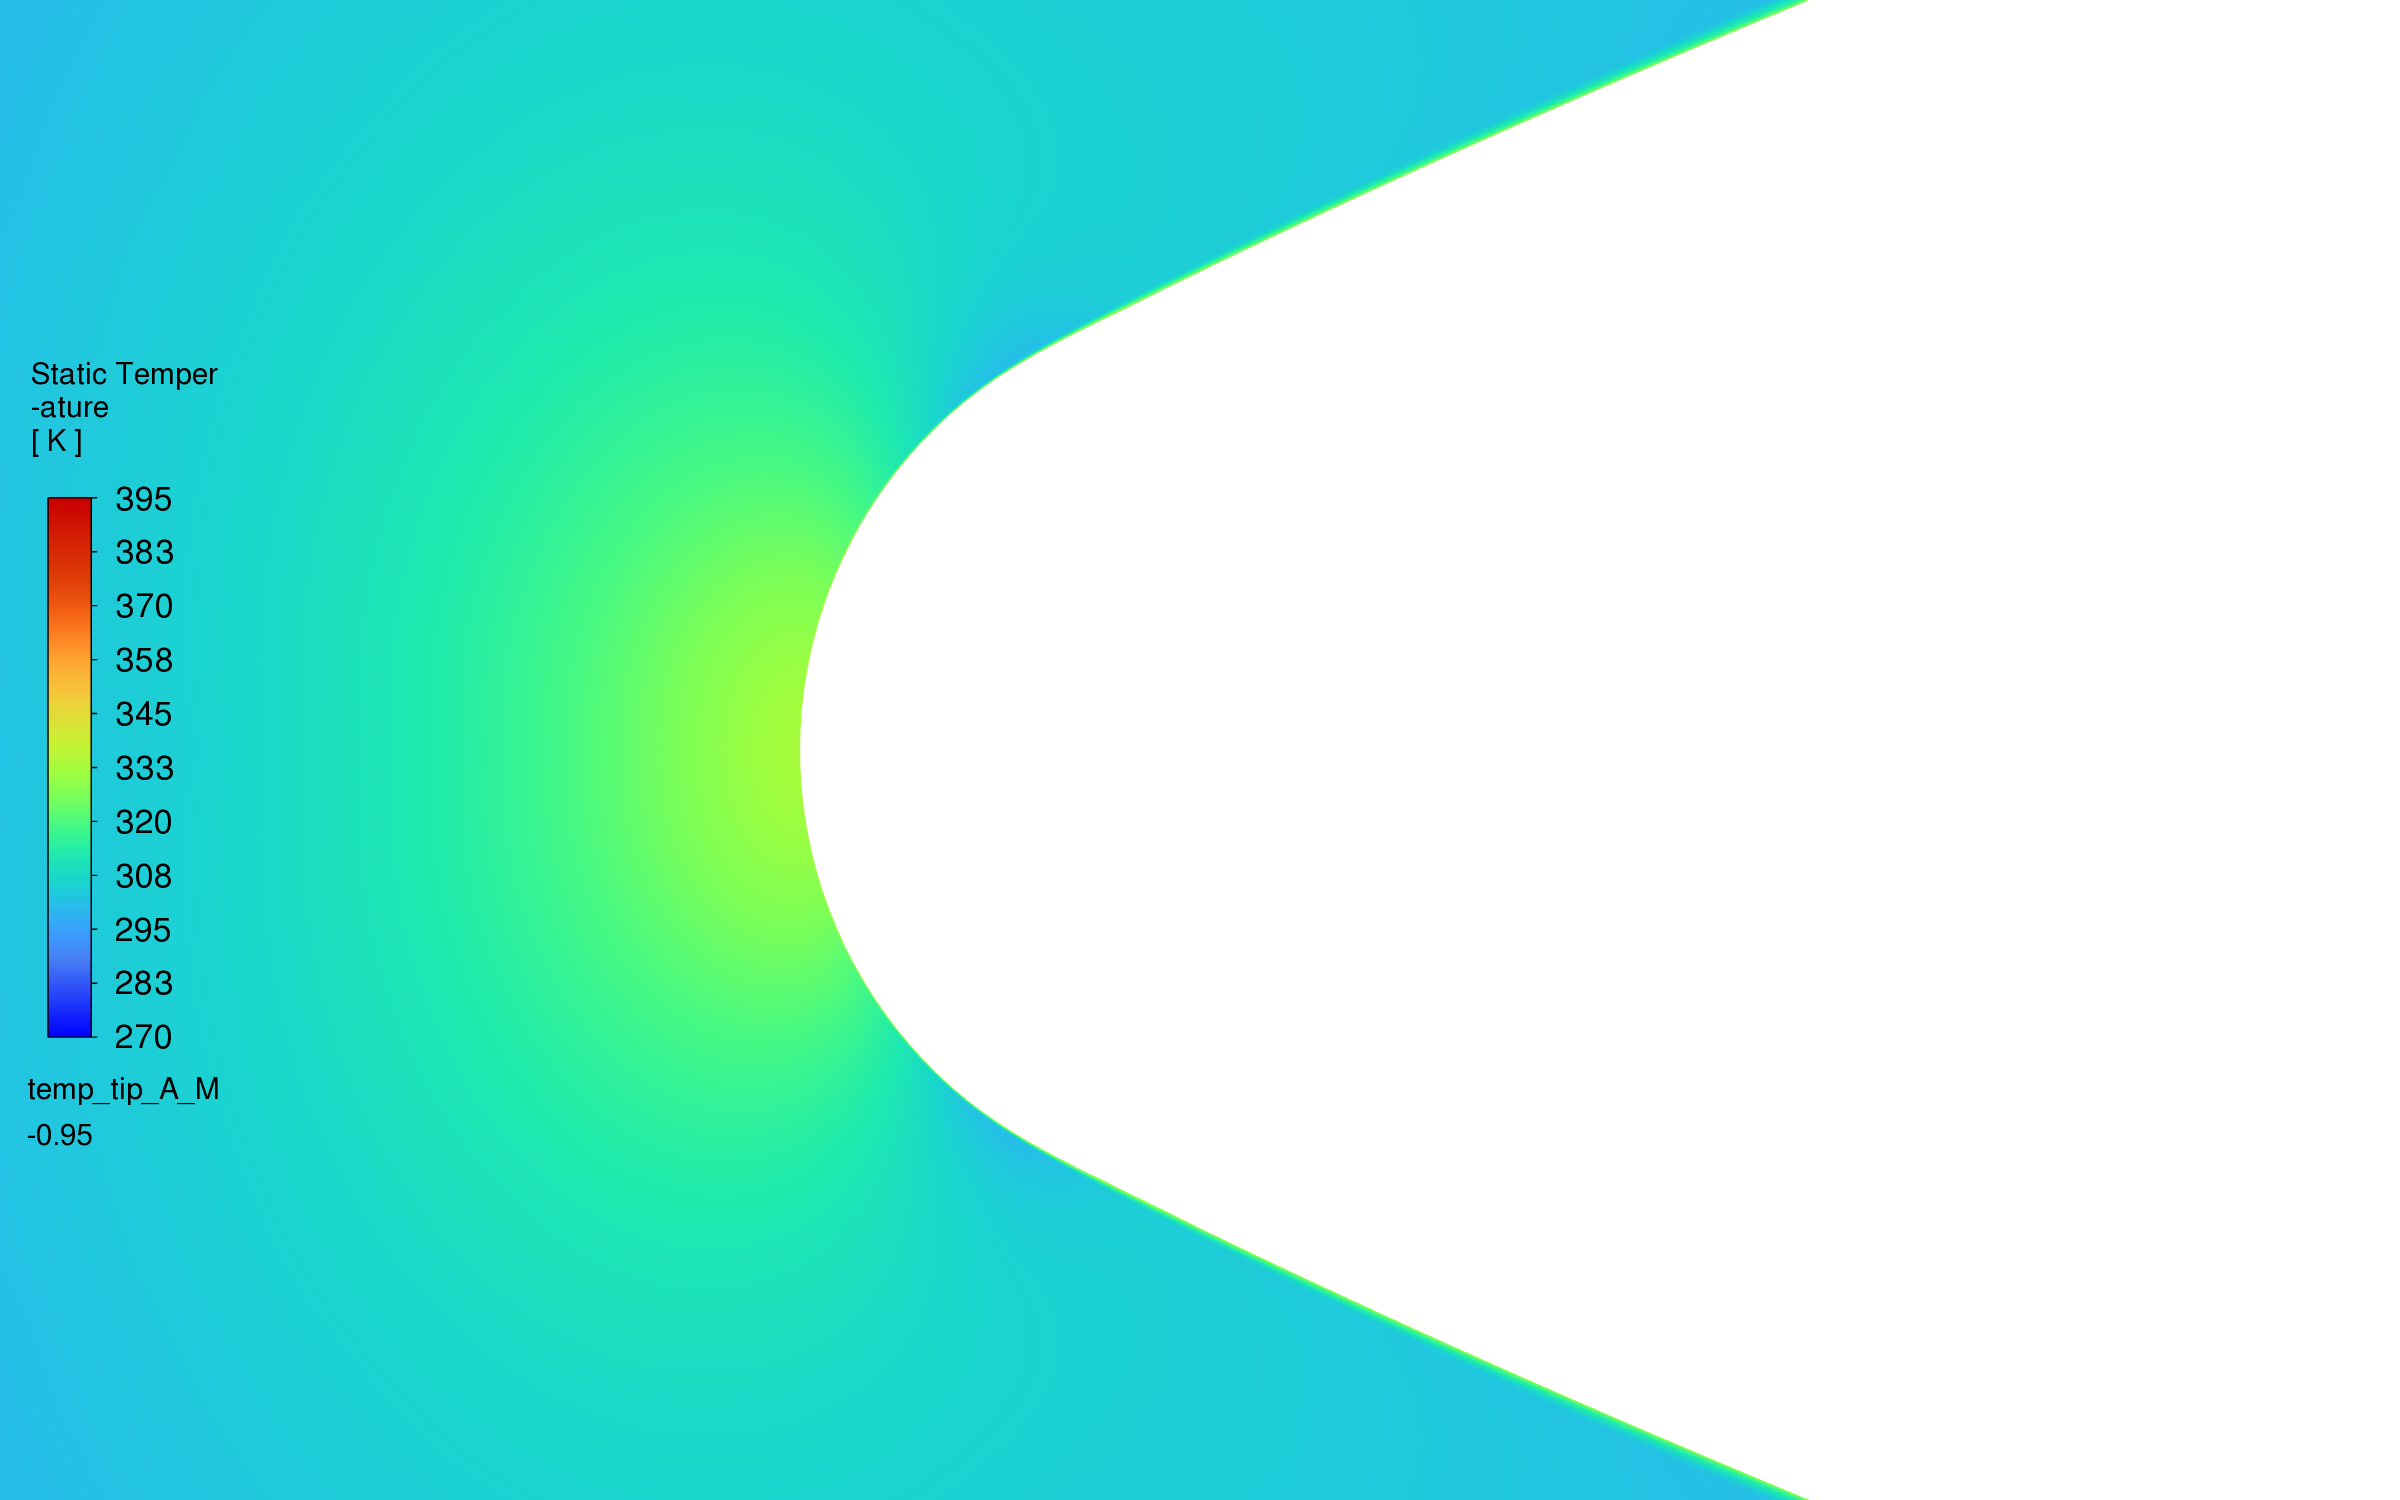
\includegraphics[width=\linewidth]{fluent_temp_tip_A_M0.95}
\caption{A, $M = 0.95$.}
\end{subfigure}\hfill
\begin{subfigure}[t]{0.325\linewidth}
\centering
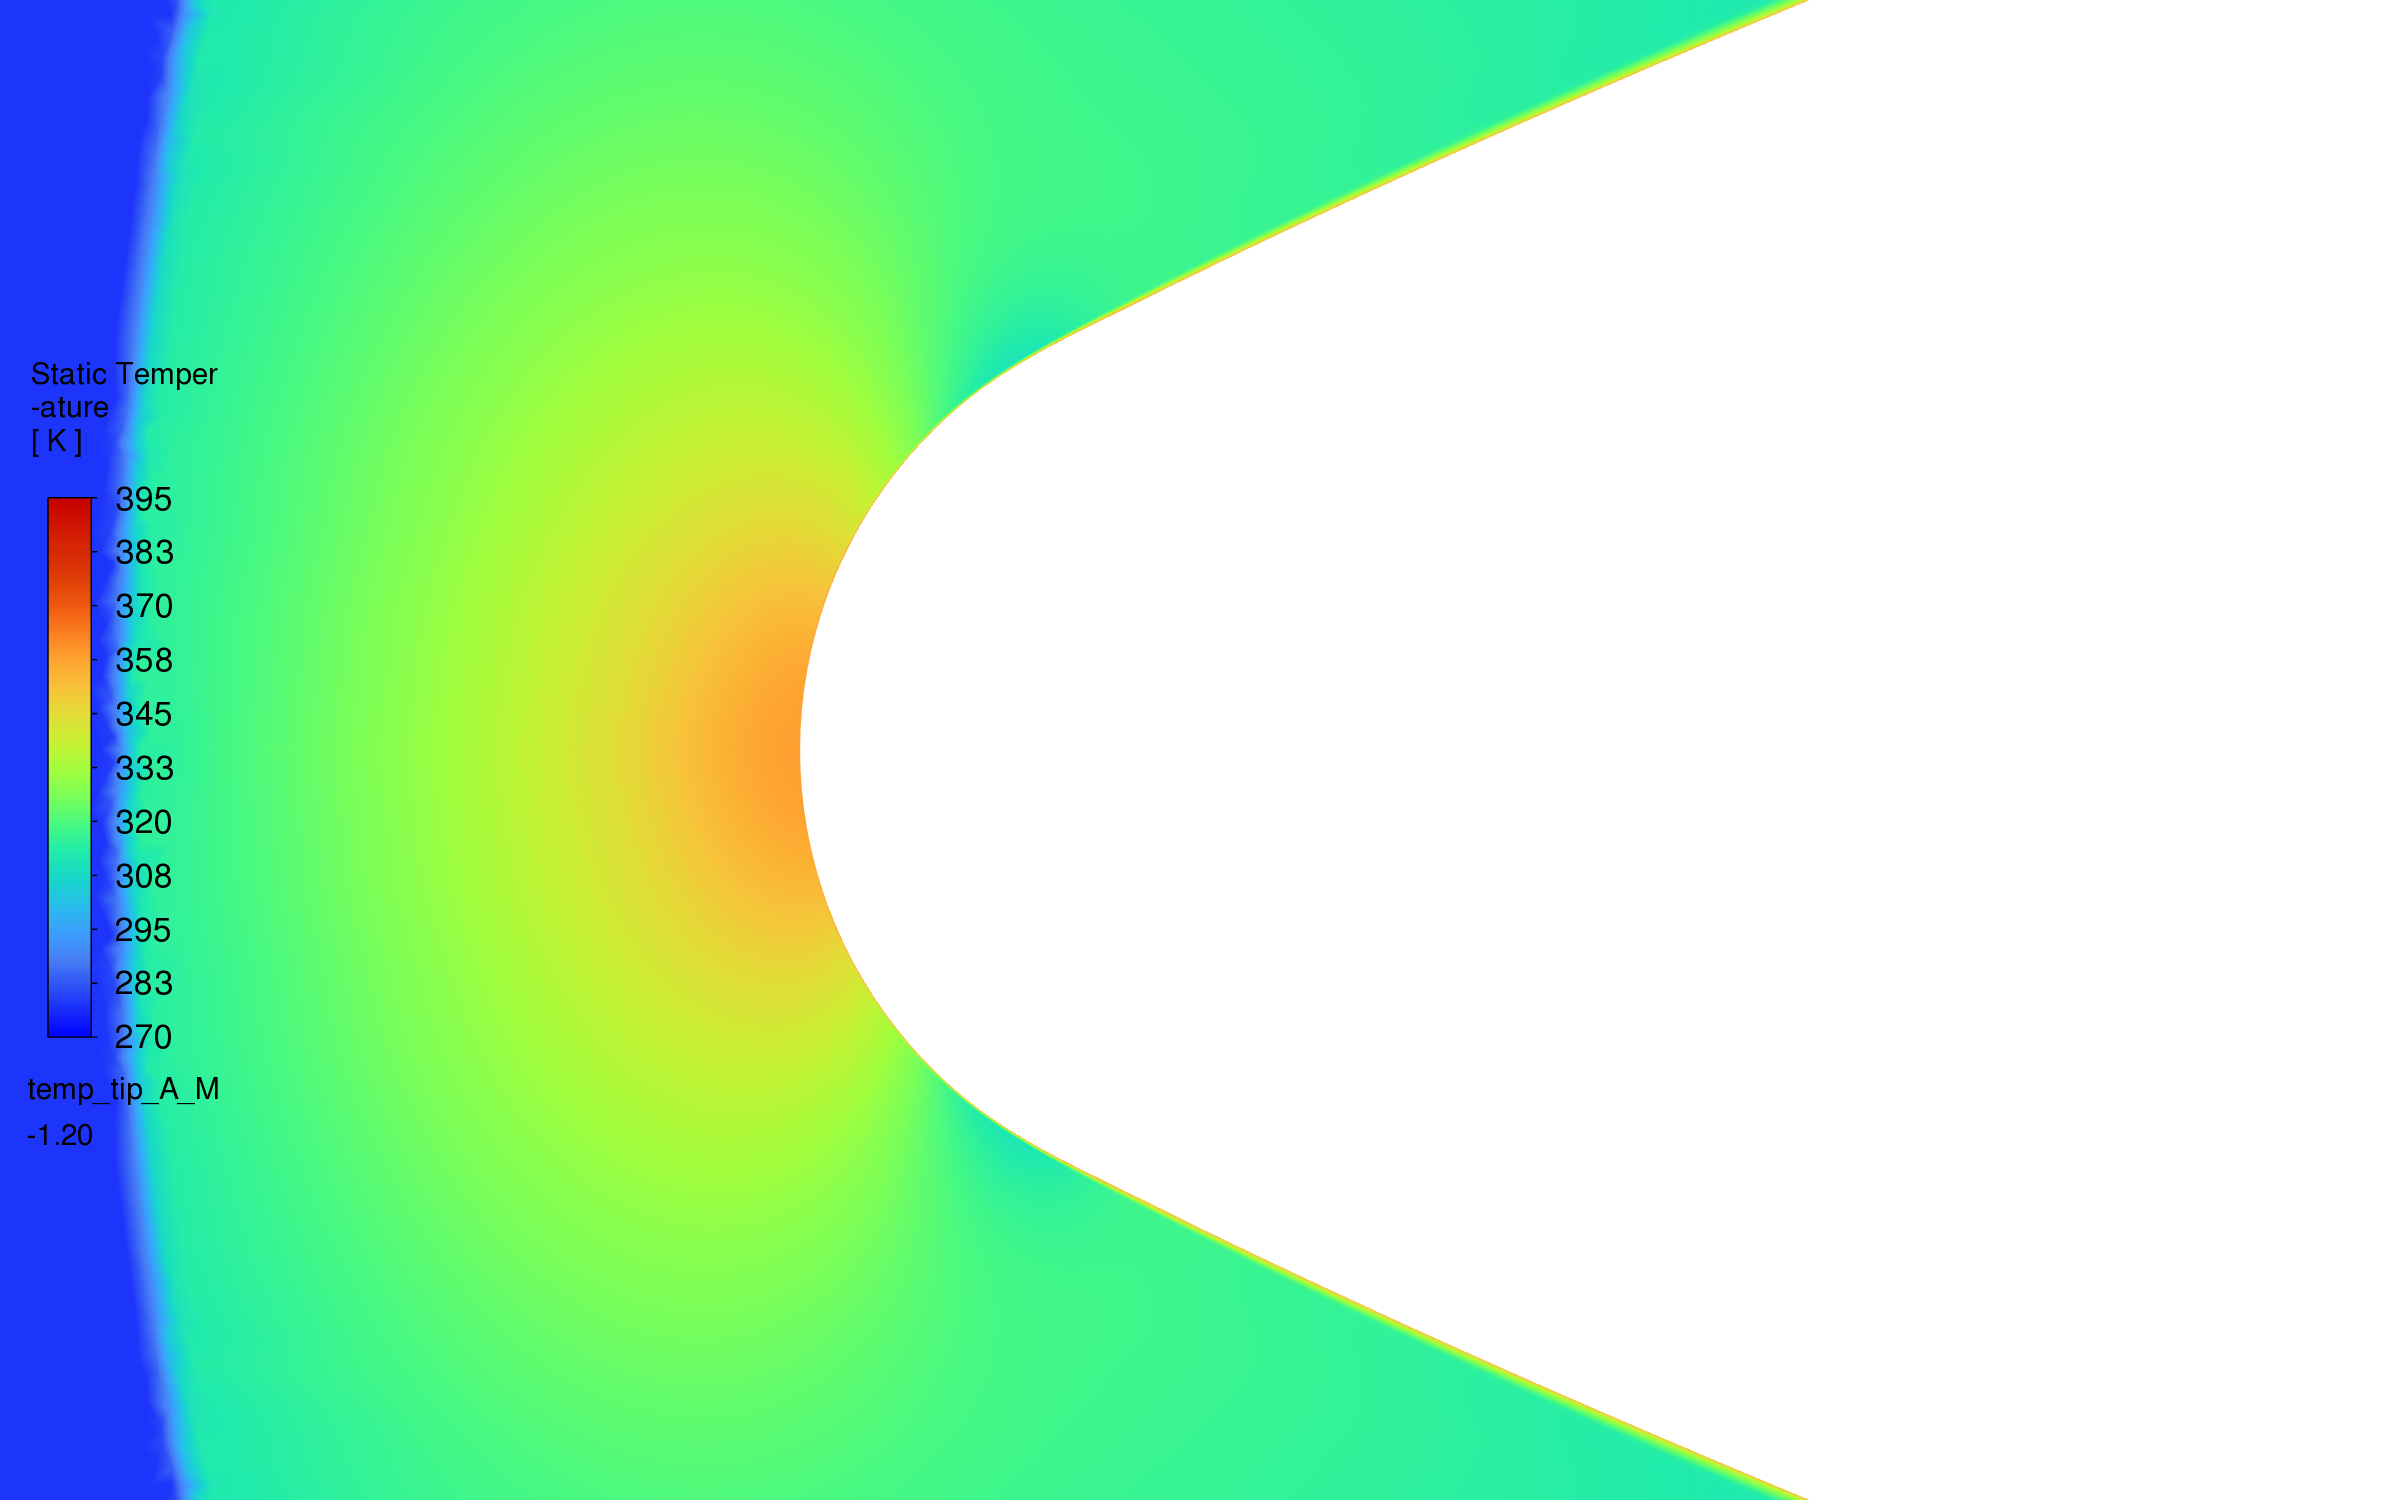
\includegraphics[width=\linewidth]{fluent_temp_tip_A_M1.20}
\caption{A, $M = 1.20$.}
\end{subfigure}\hfill
\begin{subfigure}[t]{0.325\linewidth}
\centering
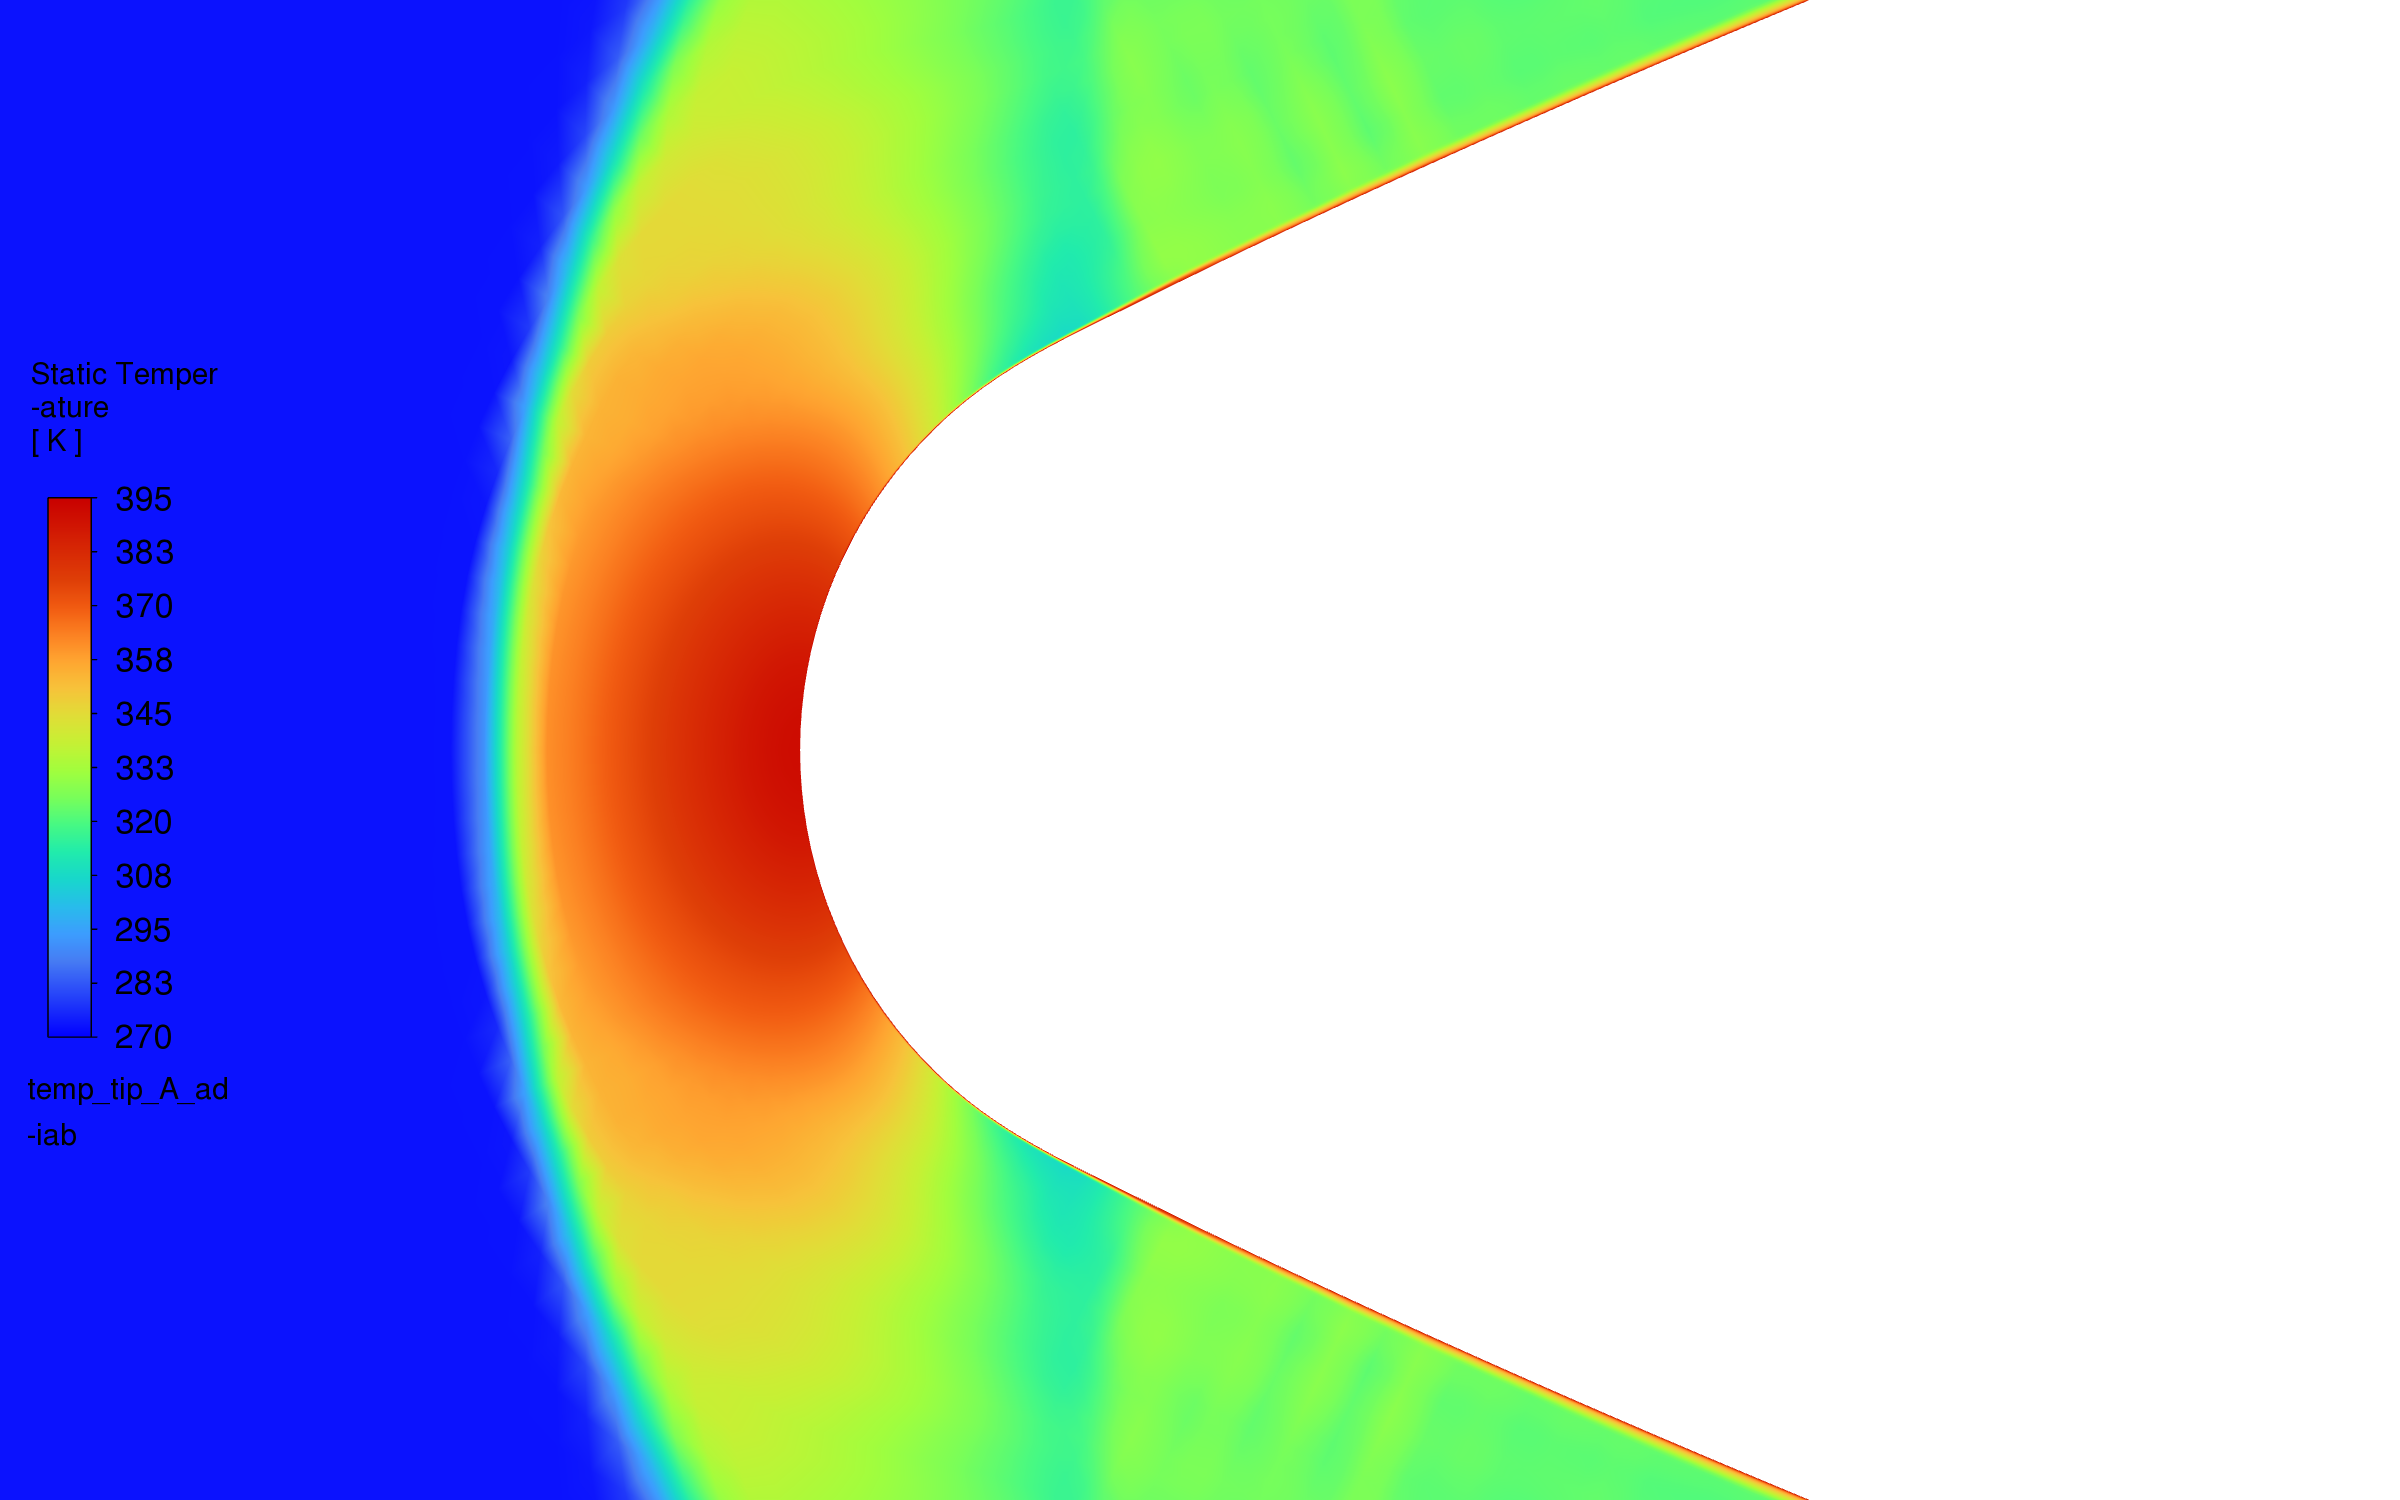
\includegraphics[width=\linewidth]{fluent_temp_tip_A_adiab}
\caption{A, burnout.}
\end{subfigure}

\smallskip
\begin{subfigure}[t]{0.325\linewidth}
\centering
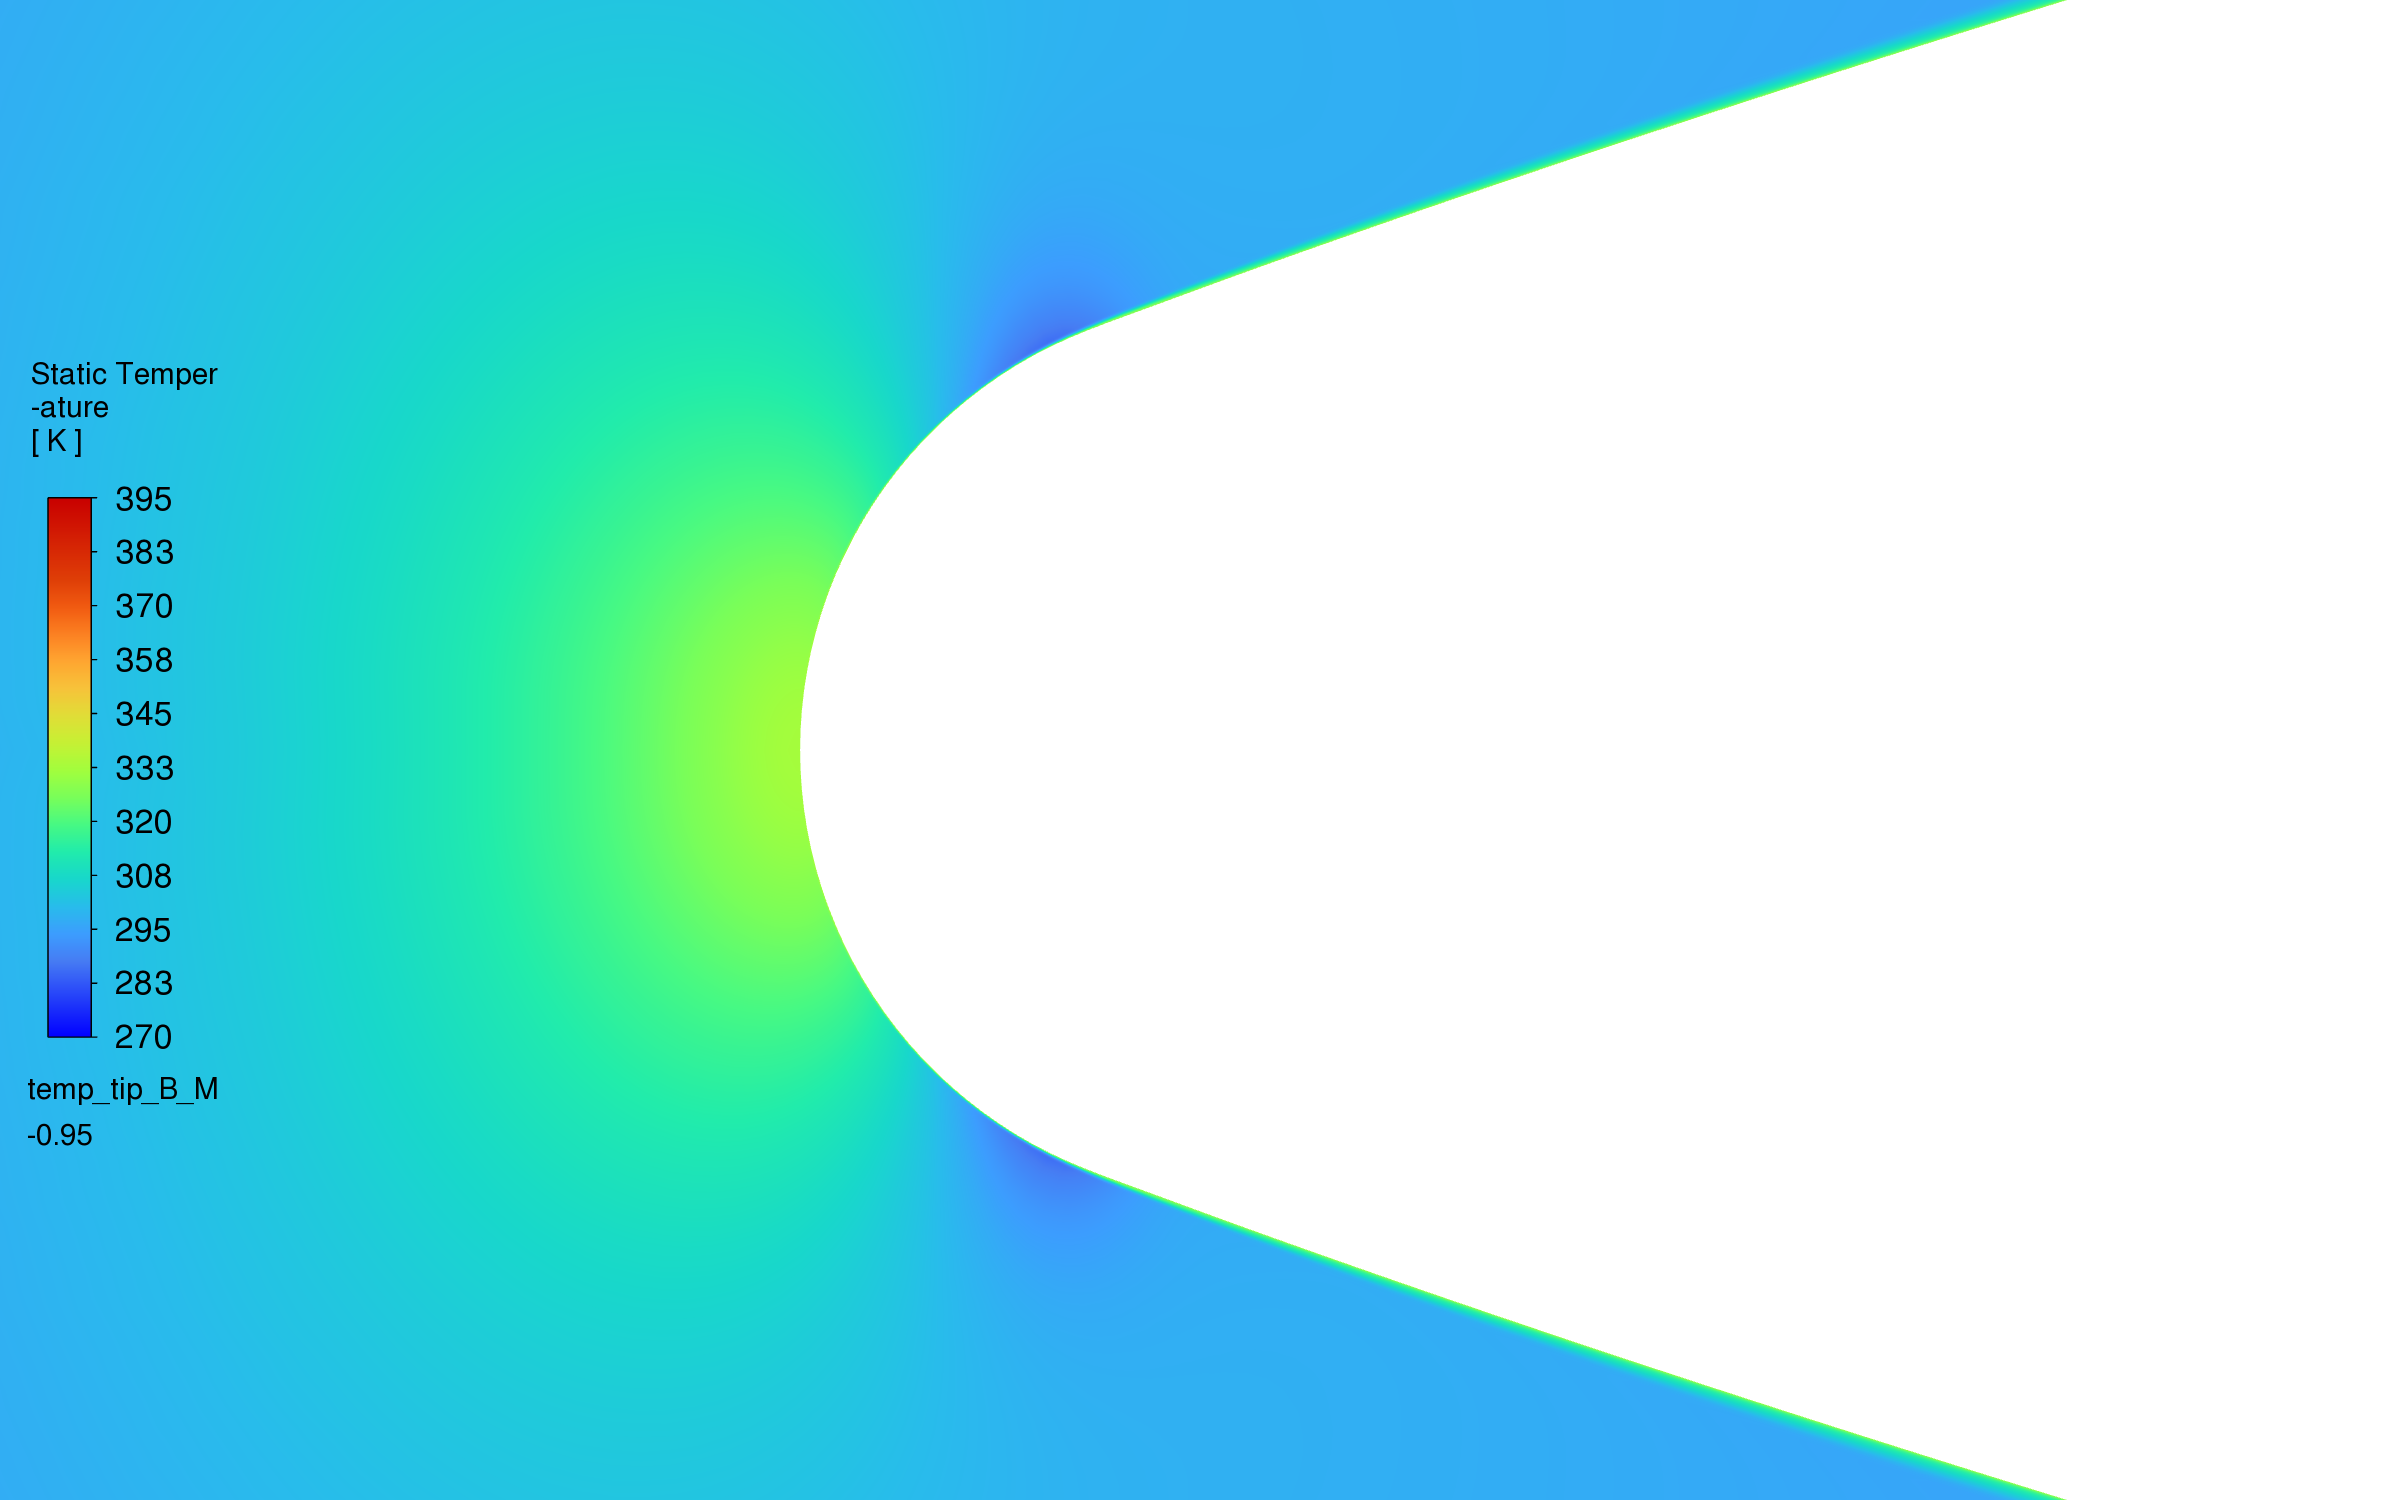
\includegraphics[width=\linewidth]{fluent_temp_tip_B_M0.95}
\caption{B, $M = 0.95$.}
\end{subfigure}\hfill
\begin{subfigure}[t]{0.325\linewidth}
\centering
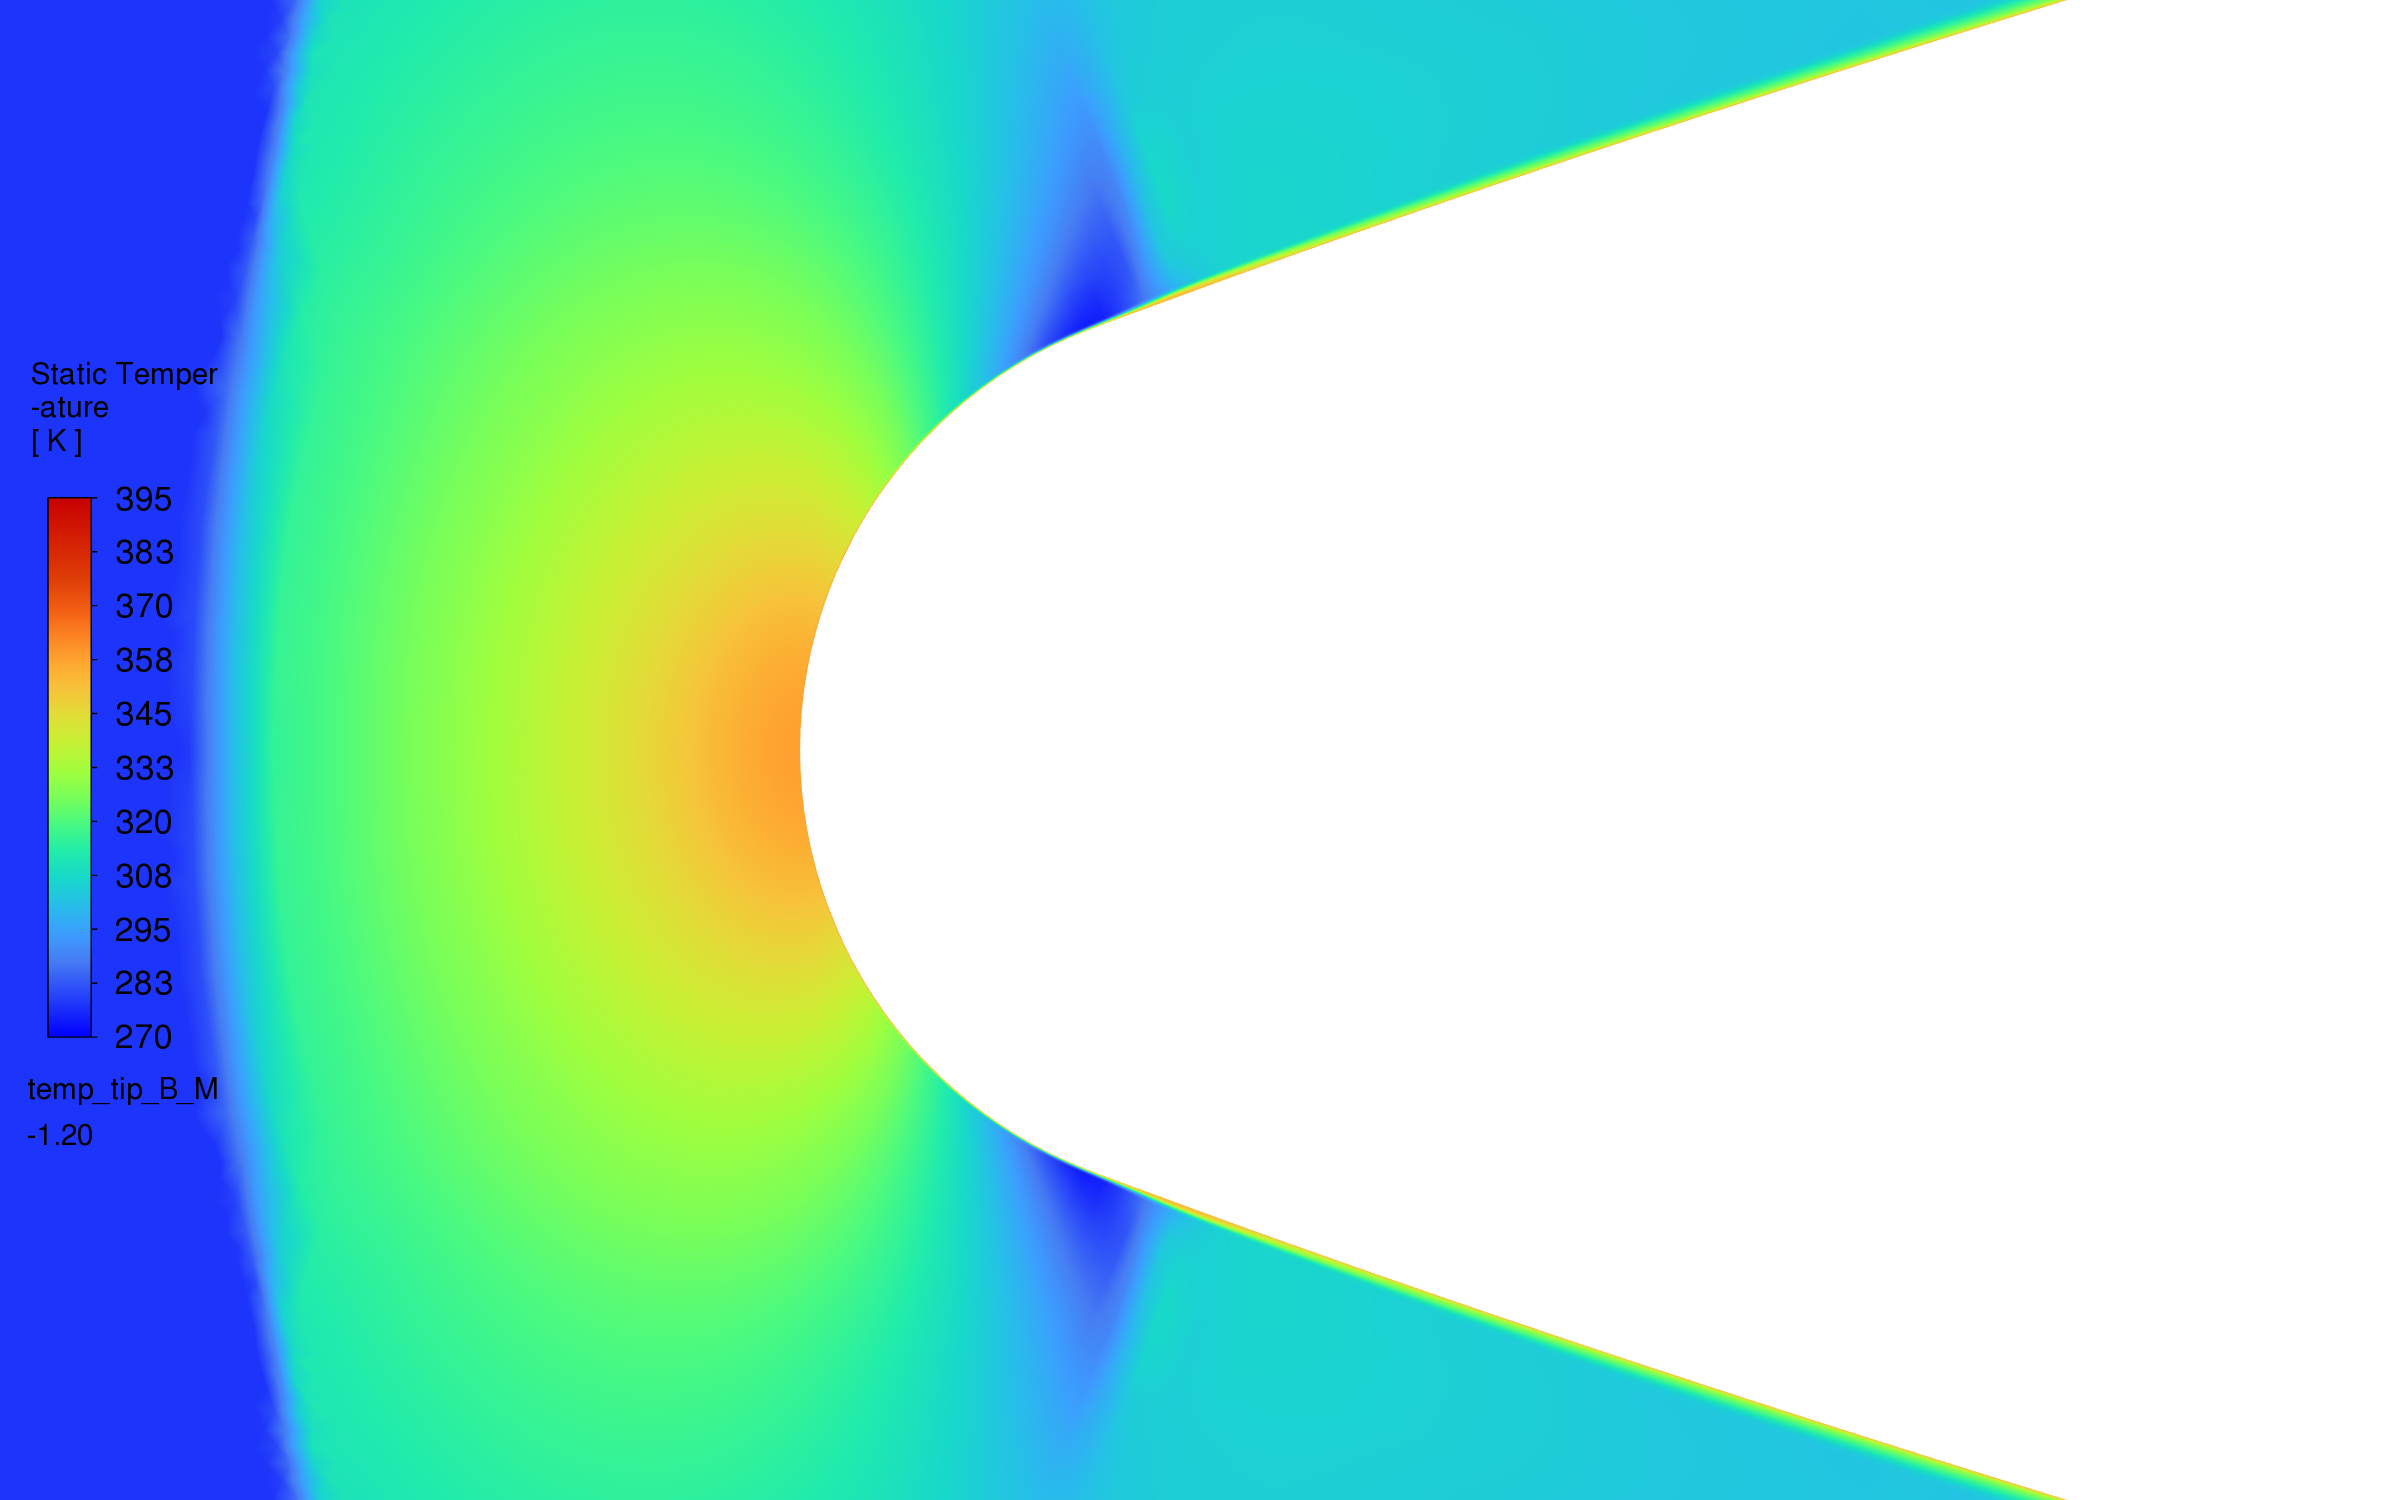
\includegraphics[width=\linewidth]{fluent_temp_tip_B_M1.20}
\caption{B, $M = 1.20$.}
\end{subfigure}\hfill
\begin{subfigure}[t]{0.325\linewidth}
\centering
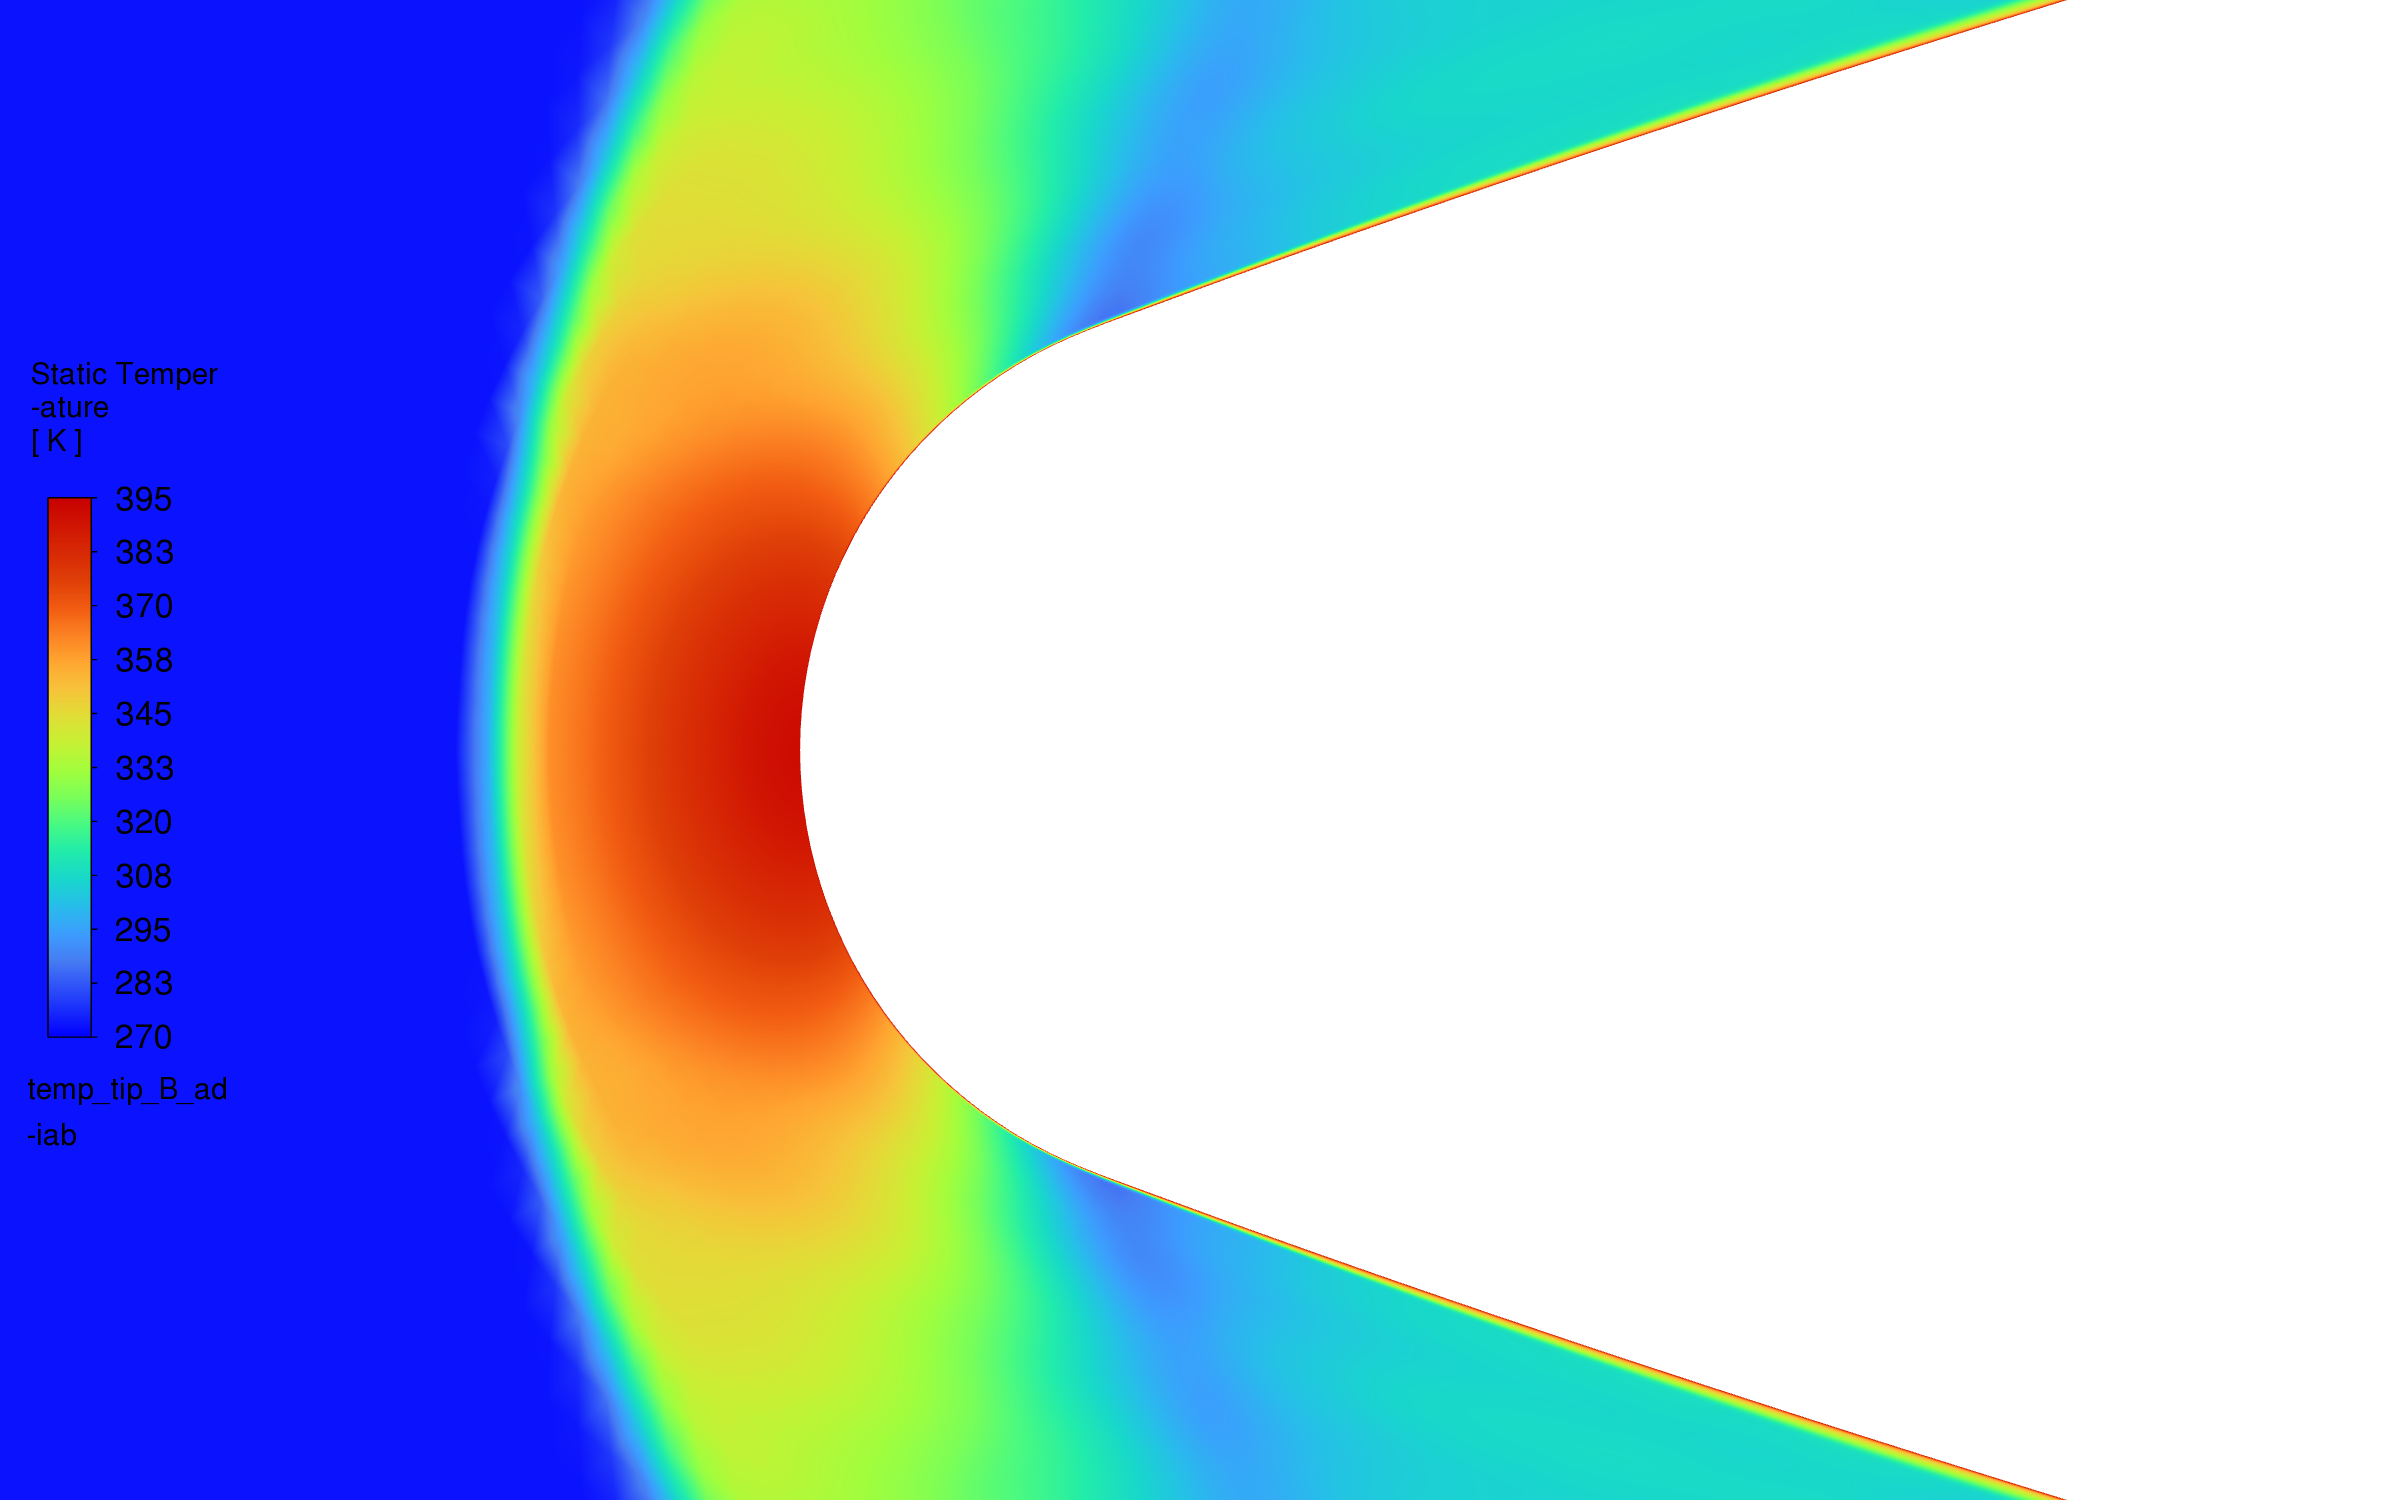
\includegraphics[width=\linewidth]{fluent_temp_tip_B_adiab}
\caption{B, burnout.}
\end{subfigure}
\caption{Air temperature around the tip at the three Fluent points of the climb (left to right: $M = 0.95$,
1.20 and burnout, $M = \val{pt-M147-M}$), adiabatic wall; top: design A, bottom: design B. Same colour
scale in all: 270\,K (blue) to 395\,K (red). The air at the tip heats up from about 333\,K to 359\,K and
391\,K.}
\label{fig:tiptemp}
\end{figure}

\begin{figure}[H]
\centering
\begin{subfigure}[t]{0.49\linewidth}
\centering
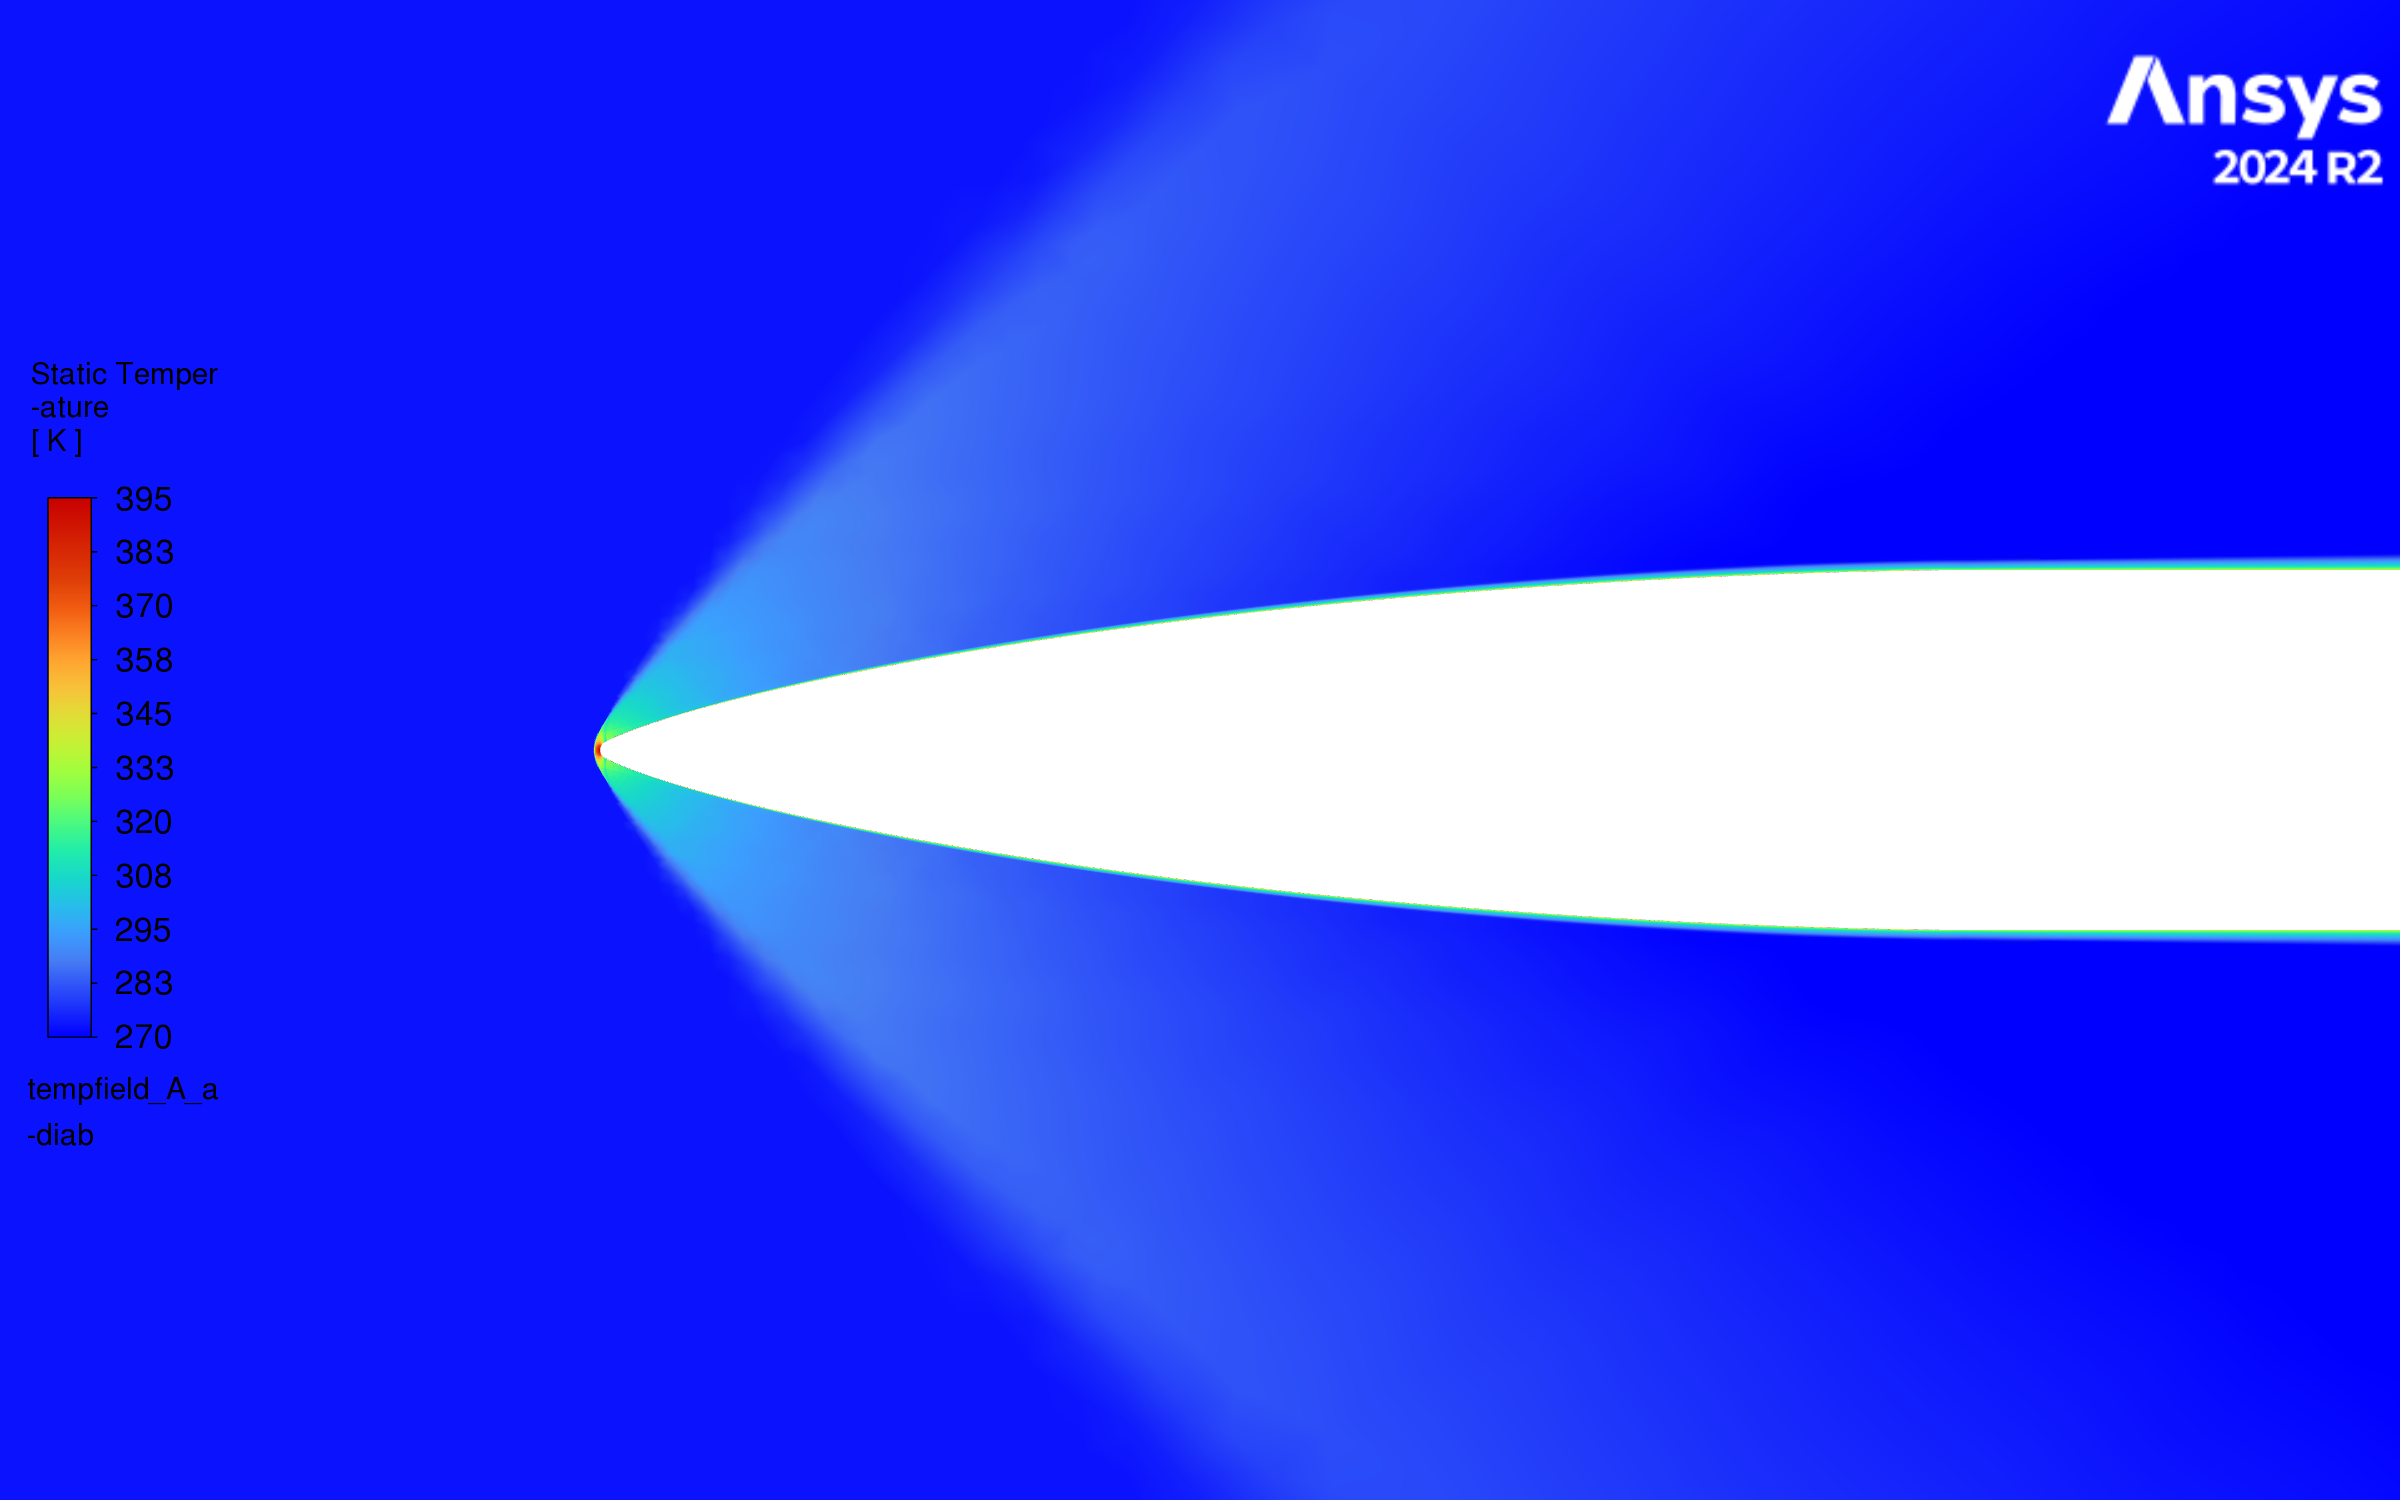
\includegraphics[width=\linewidth]{fluent_tempfield_A_adiab}
\caption{Design A.}
\end{subfigure}\hfill
\begin{subfigure}[t]{0.49\linewidth}
\centering
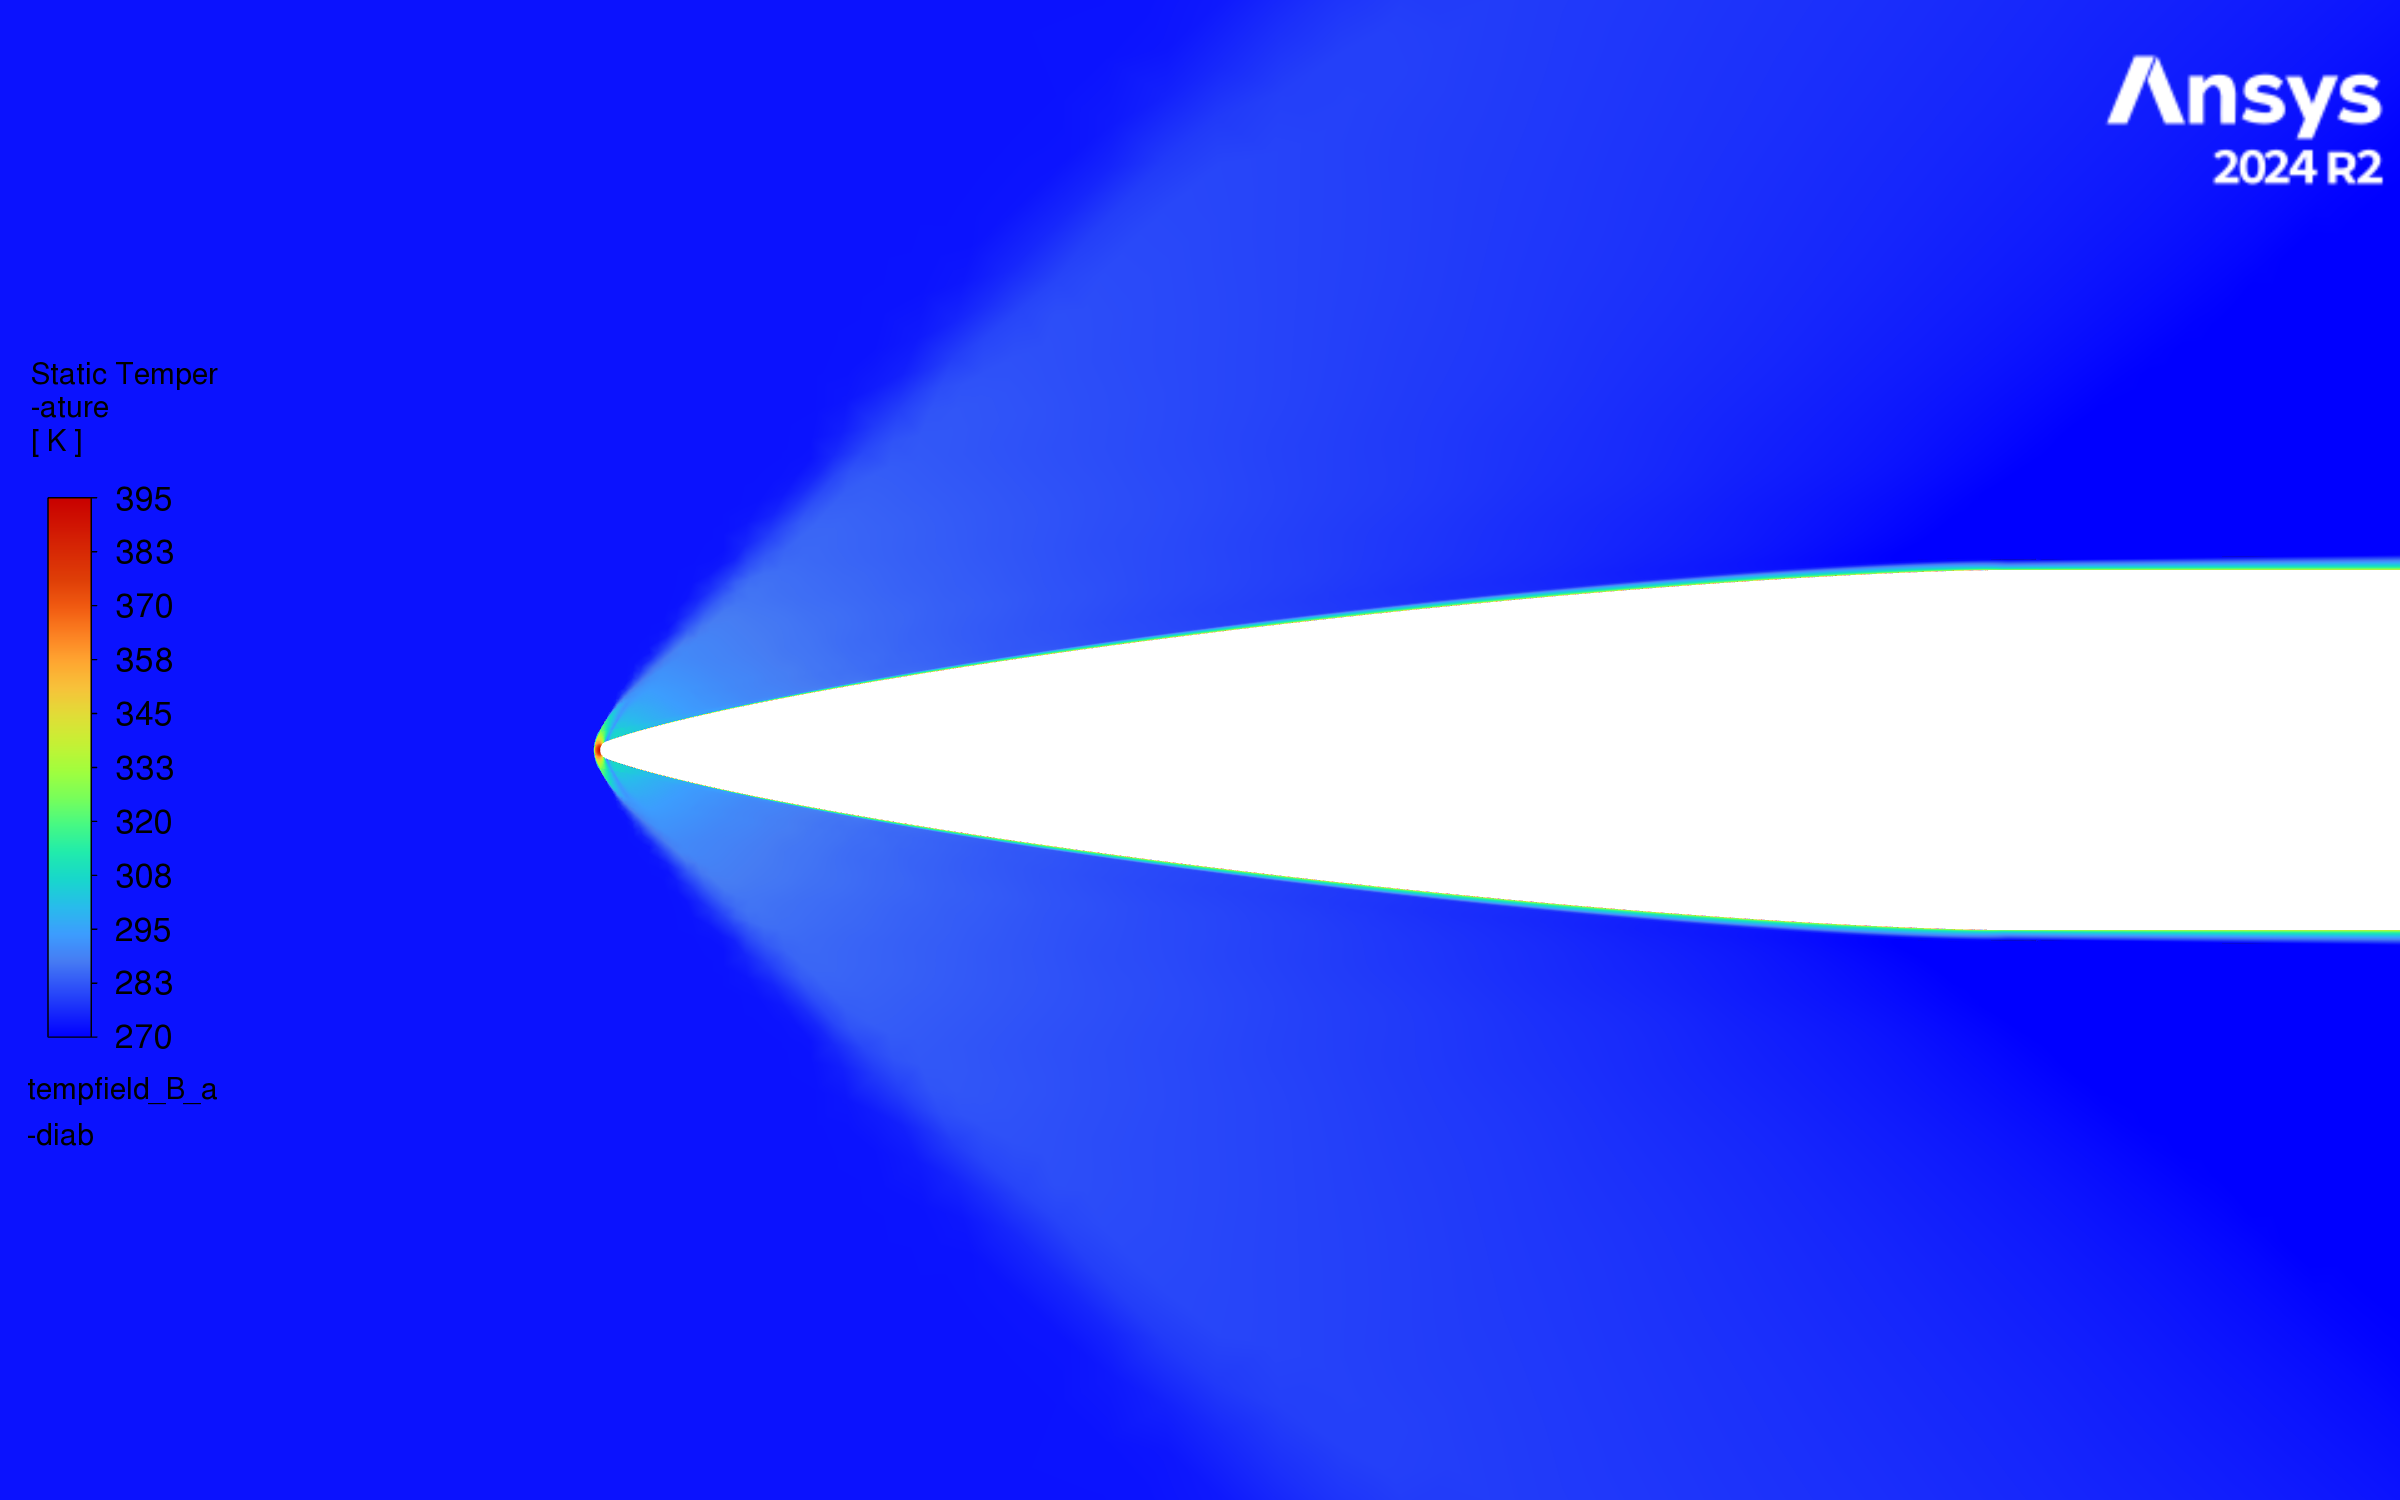
\includegraphics[width=\linewidth]{fluent_tempfield_B_adiab}
\caption{Design B.}
\end{subfigure}
\caption{Air temperature around the whole nose at burnout, adiabatic wall (Fluent). The hot air stays in a
thin layer along the wall; the light band is the air heated by the bow shock. Colour scale: 270\,K (blue) to 395\,K (red).}
\label{fig:tempfield}
\end{figure}

\begin{figure}[H]
\centering
\begin{subfigure}[t]{0.49\linewidth}
\centering
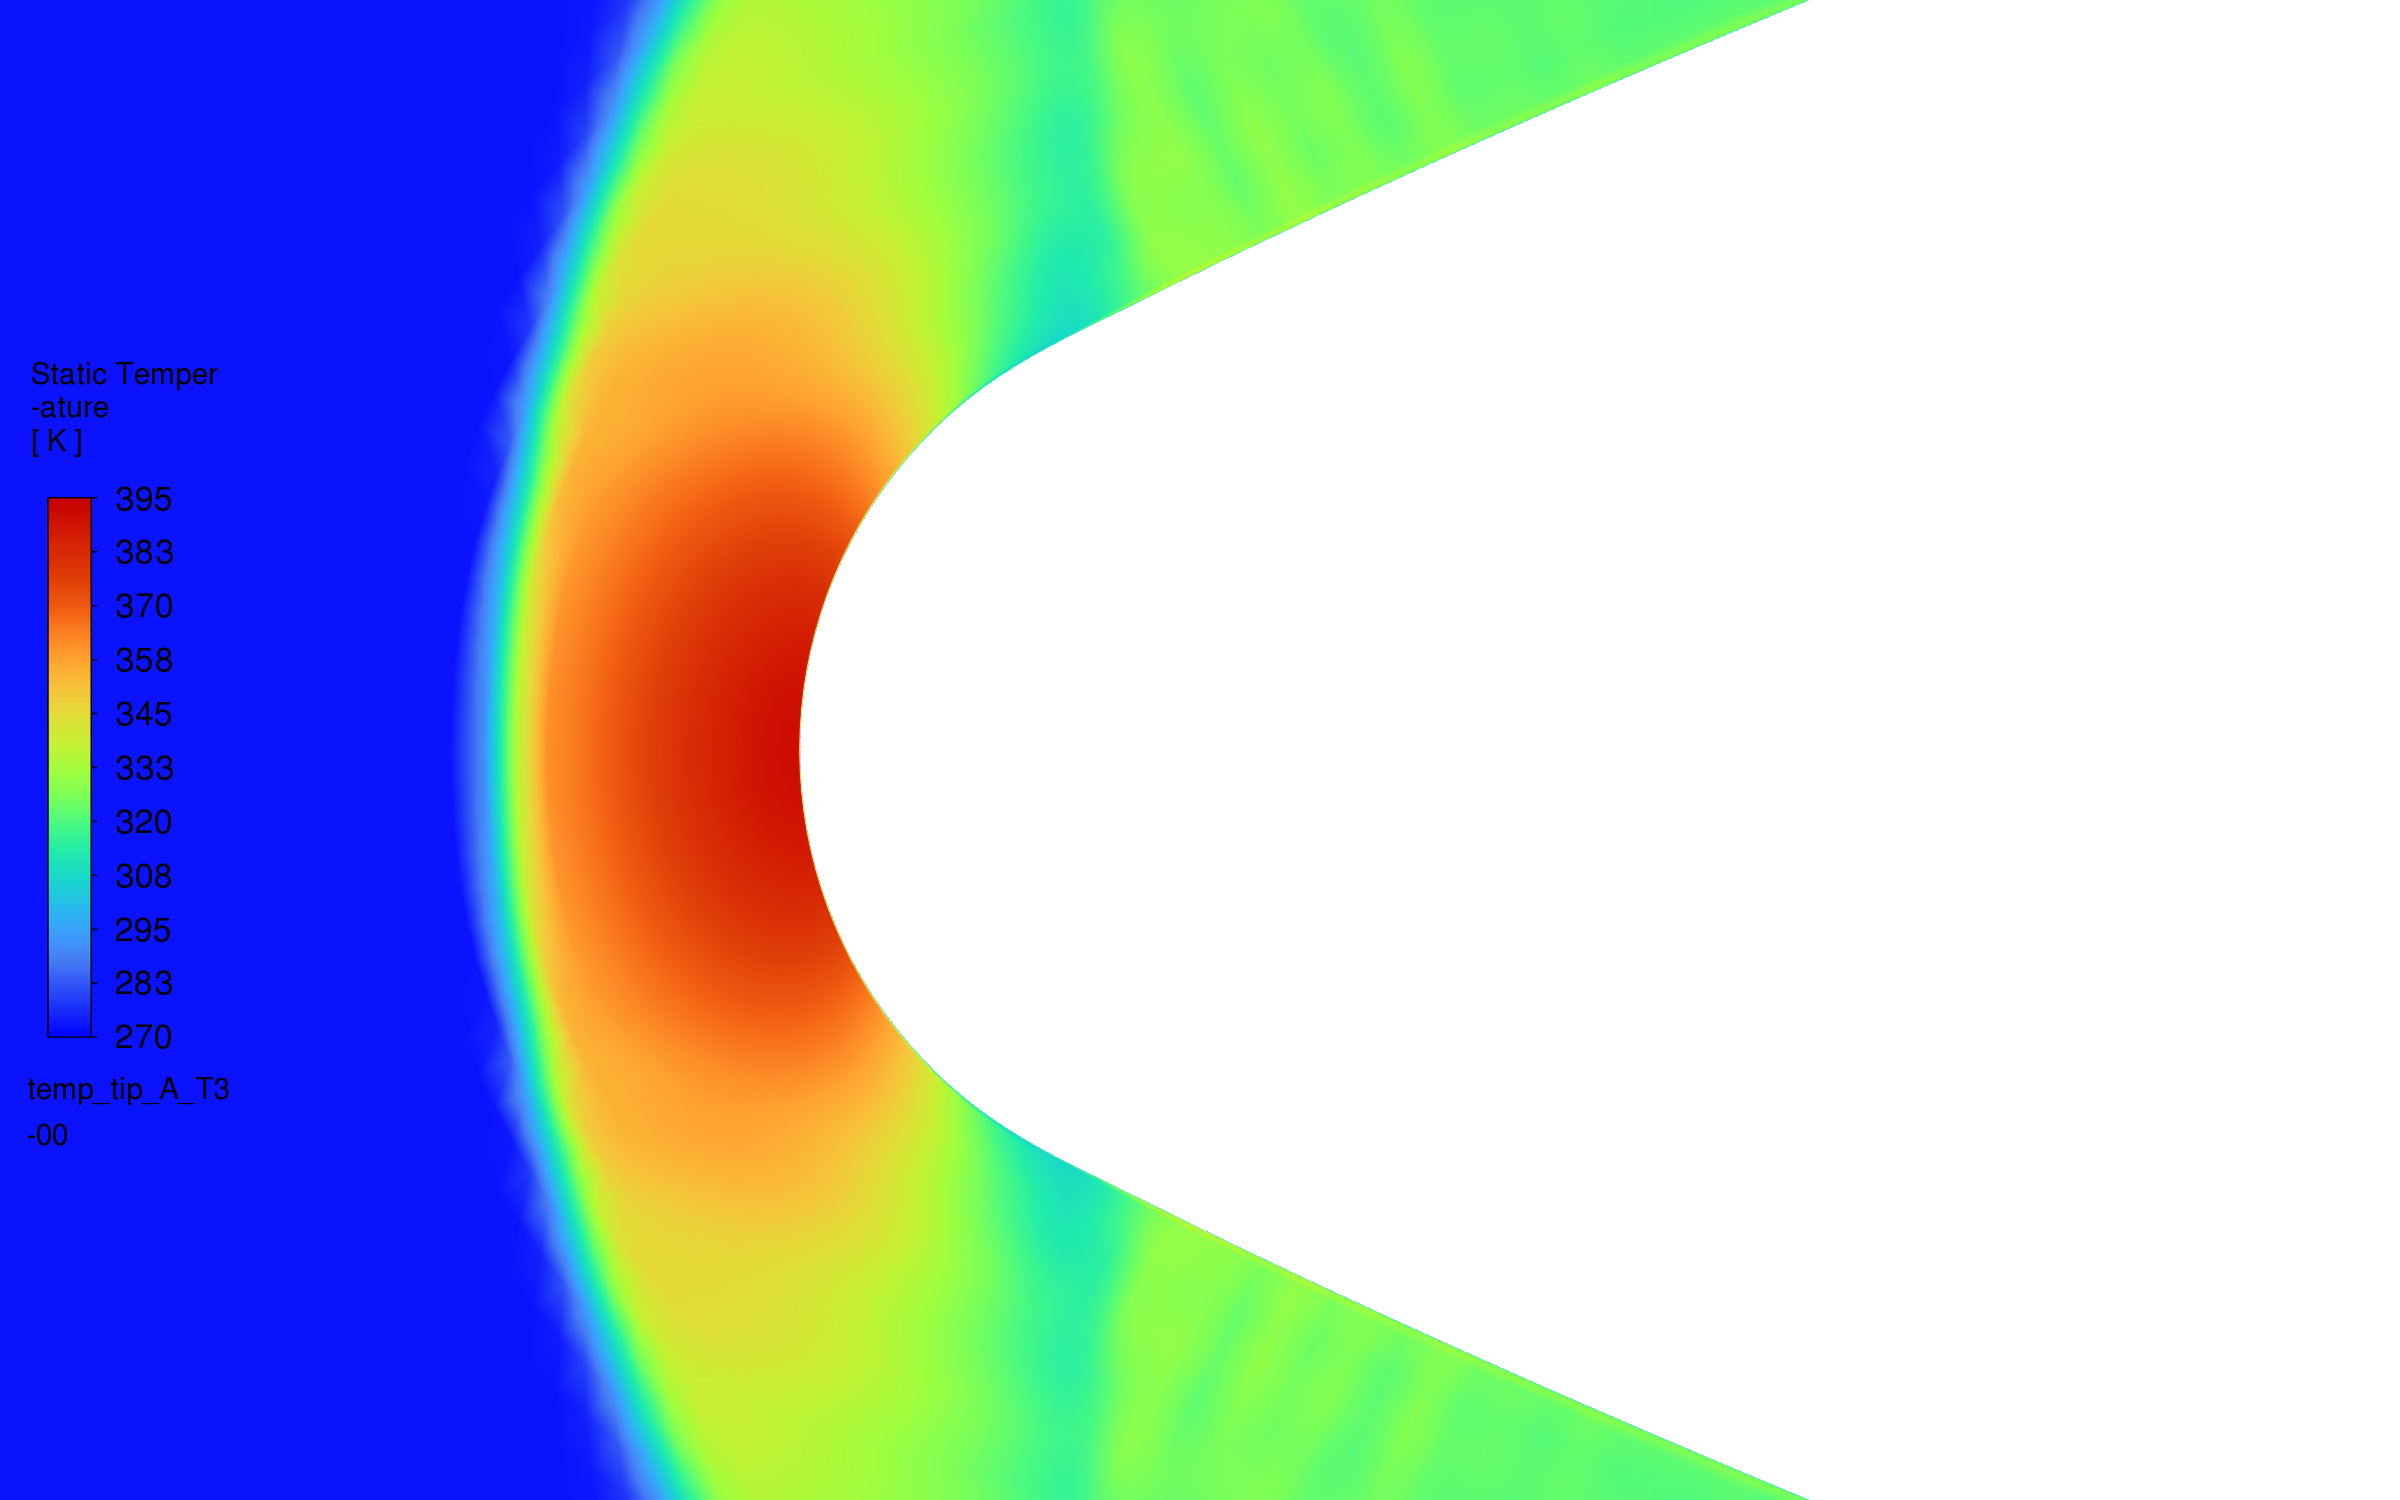
\includegraphics[width=\linewidth]{fluent_temp_tip_A_T300}
\caption{Design A.}
\end{subfigure}\hfill
\begin{subfigure}[t]{0.49\linewidth}
\centering
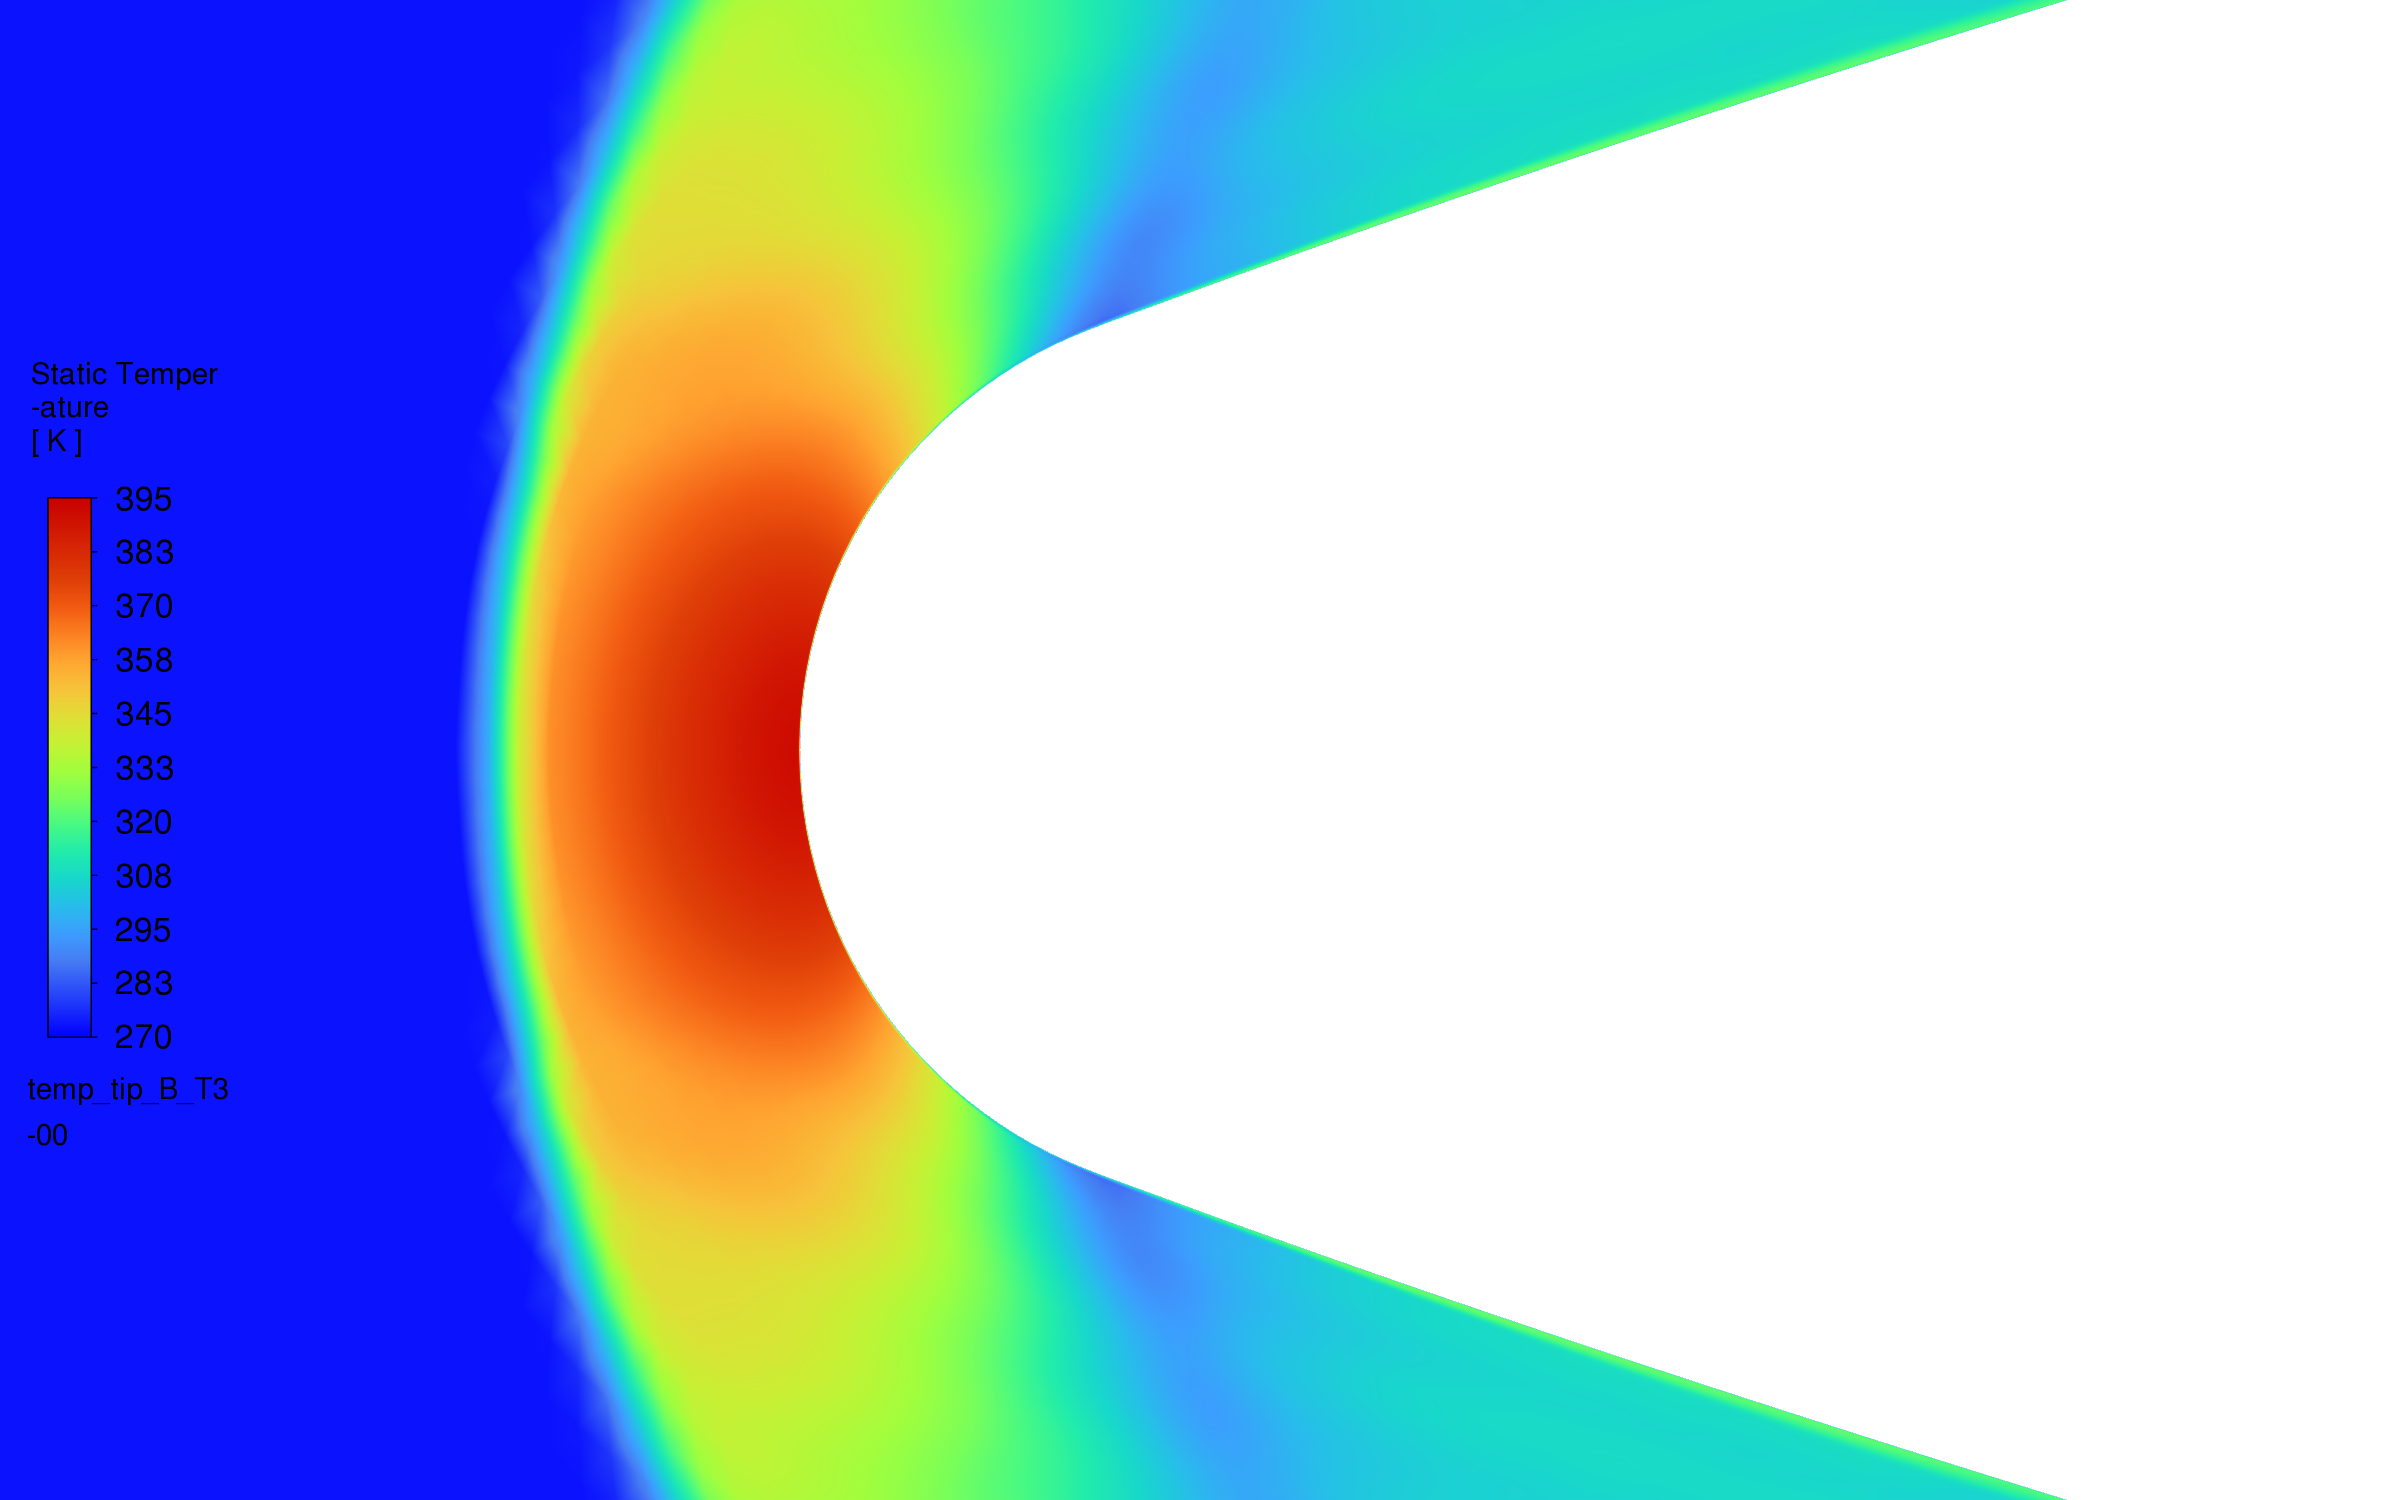
\includegraphics[width=\linewidth]{fluent_temp_tip_B_T300}
\caption{Design B.}
\end{subfigure}
\caption{Air temperature around the tip at burnout with the wall held at \SI{300}{K} (Fluent). The cold
wall cools the air next to it: this temperature drop at the wall is the heat going into the nose. Colour scale: 270\,K (blue) to 395\,K (red).}
\label{fig:tipT300}
\end{figure}

\paragraph{Heating along the wall.} Figures~\ref{fig:taw}--\ref{fig:hfluent} give the heating along the
wall of both designs, and Table~\ref{tab:fluentheat} sums it up.
\begin{itemize}
\item The \textbf{wall temperature} $T_{aw}$ is \val{A-Taw0}\,K at the tip and
\val{A-Taw-far-lo}--\val{A-Taw-far-hi}\,K further back: the whole nose is driven to about
107--110\,\si{\celsius} at burnout.
\item The \textbf{heat flux} and $h$ are highest at the tip and fall along the nose: $h$ goes from about
\SI{1900}{W/(m^2K)} at the tip to about \SI{1000}{W/(m^2K)} at 50\,mm and about \SI{550}{W/(m^2K)} at
the shoulder. So the front of the shell heats up fastest.
\item A and B differ only over the first 10\,cm, and by little. The heating does not separate the two
designs.
\end{itemize}

\begin{figure}[H]
\centering
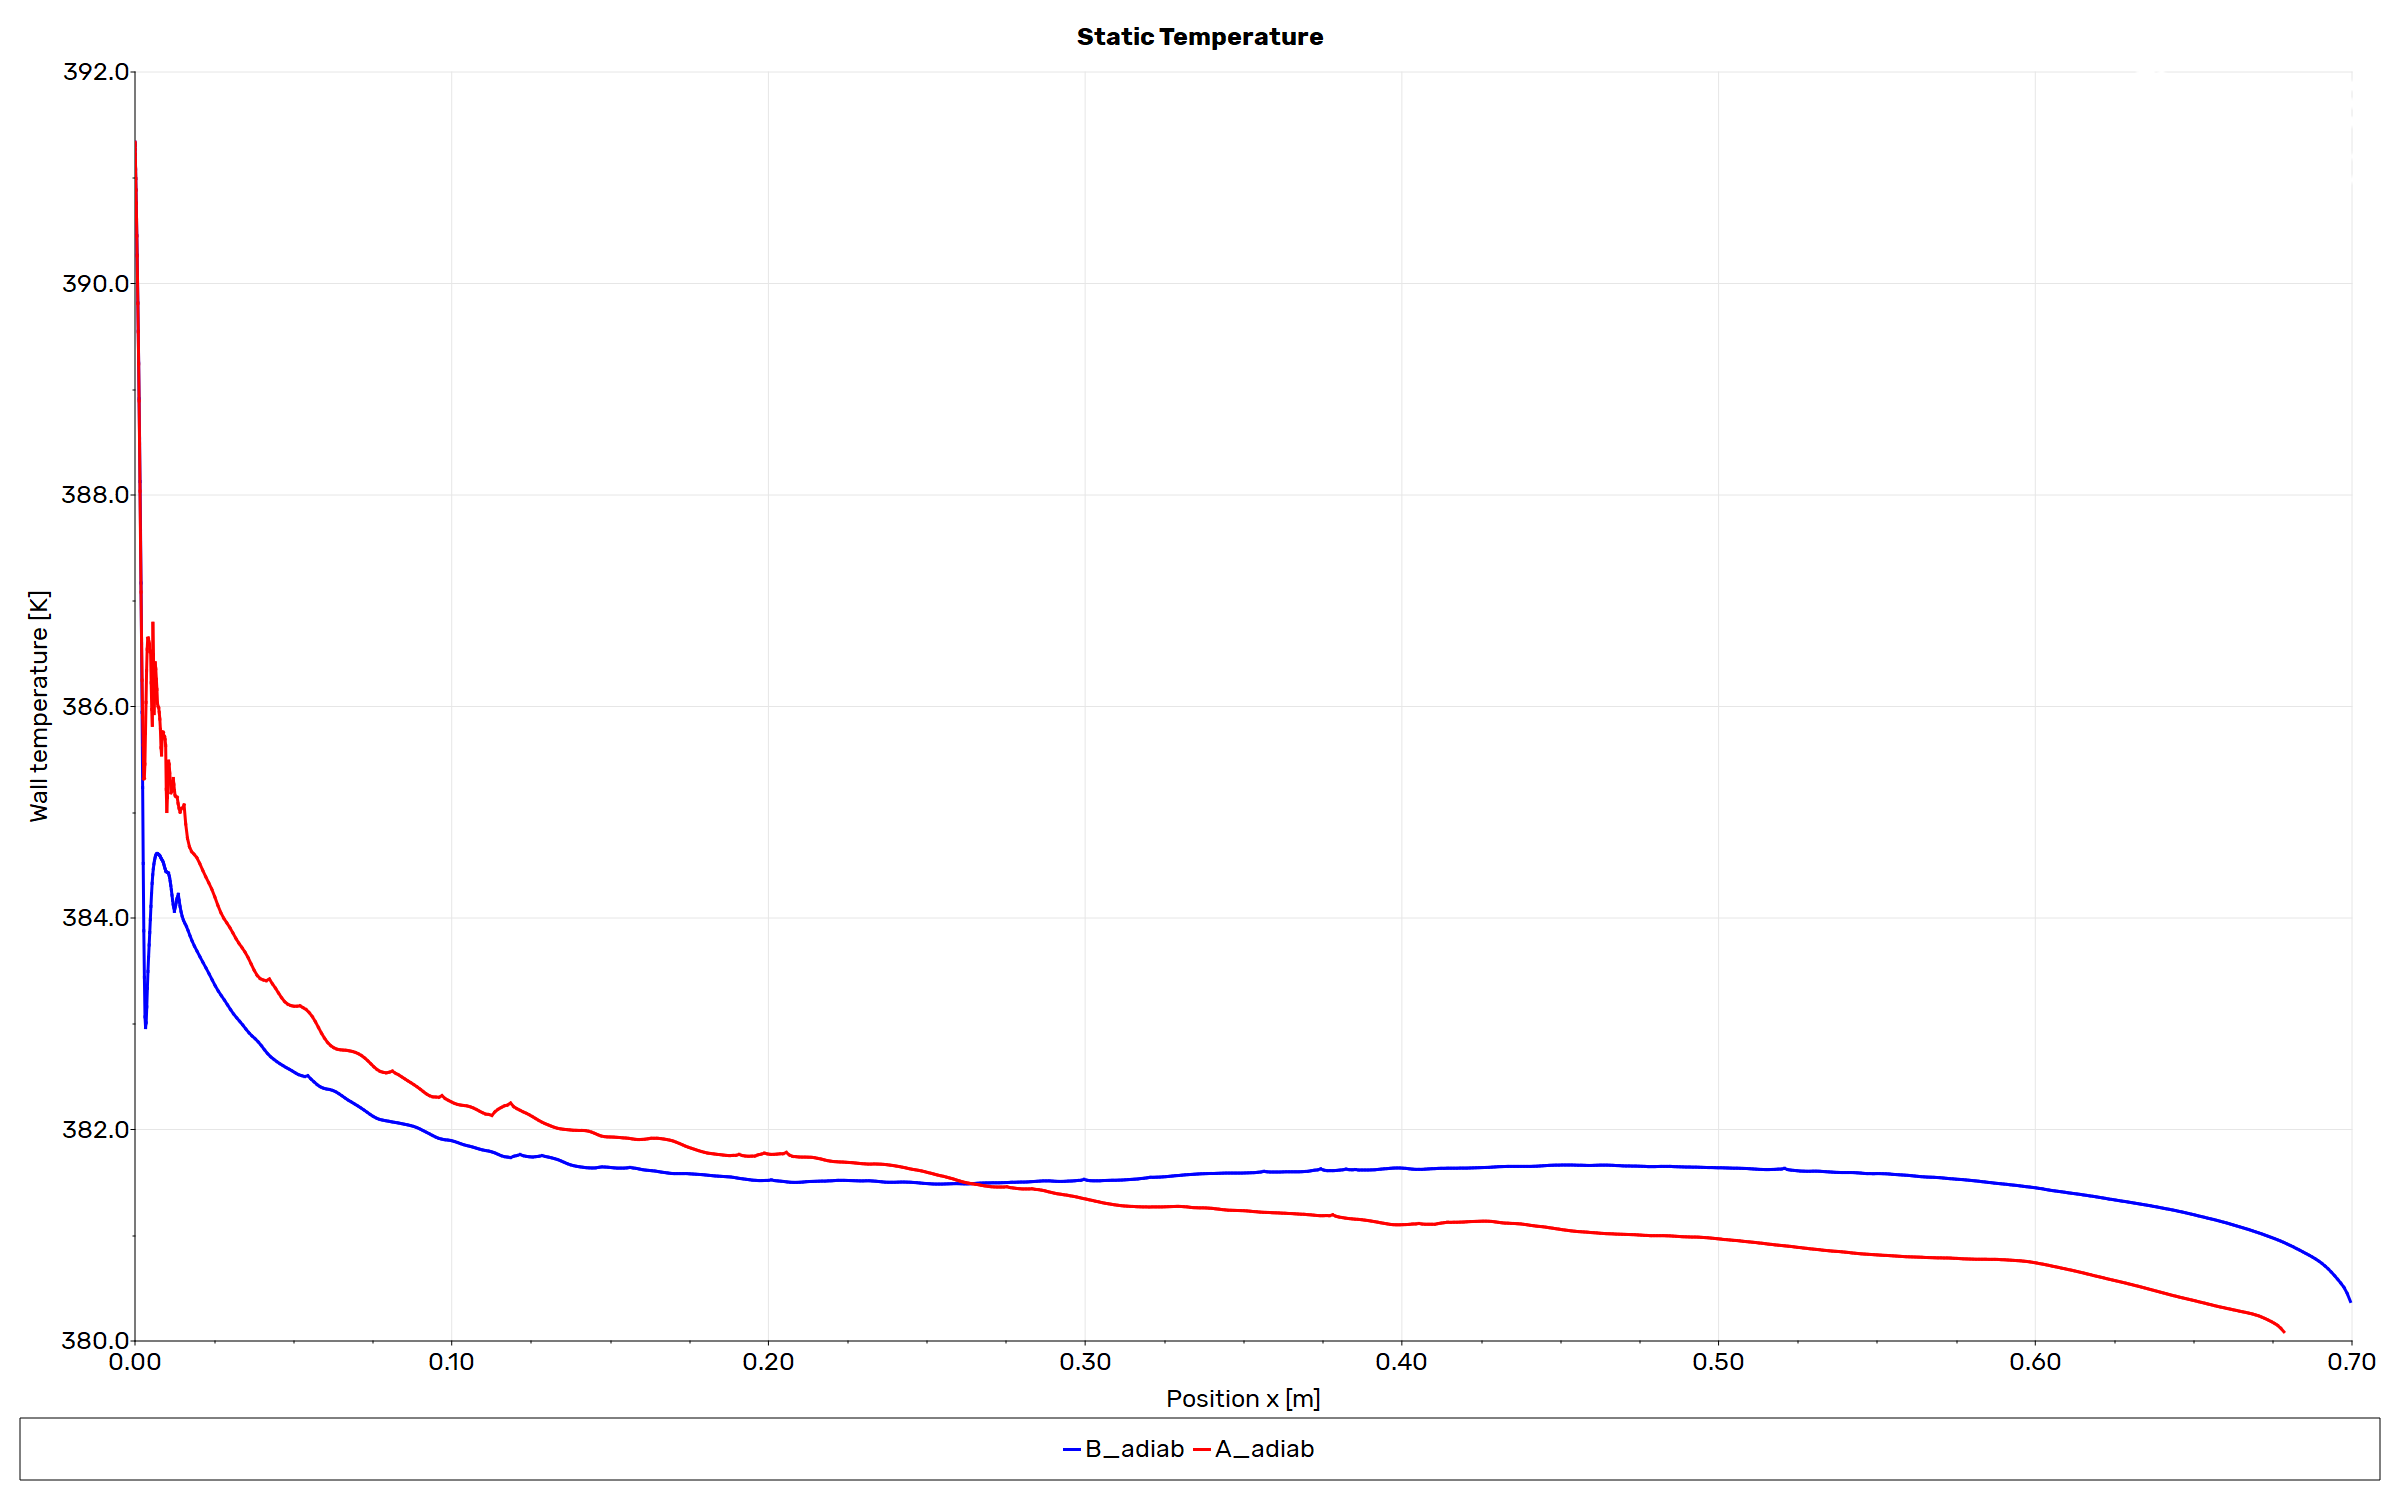
\includegraphics[width=0.9\linewidth]{fluent_twall_AB_adiab}
\caption{Adiabatic wall temperature along the nose at burnout, design A (red) and B (blue), Fluent. This
is the temperature the air drives the wall towards. The ripple over the first 15\,mm is a mesh effect,
where the fine tip cells meet the wall cells.}
\label{fig:taw}
\end{figure}

\begin{figure}[H]
\centering
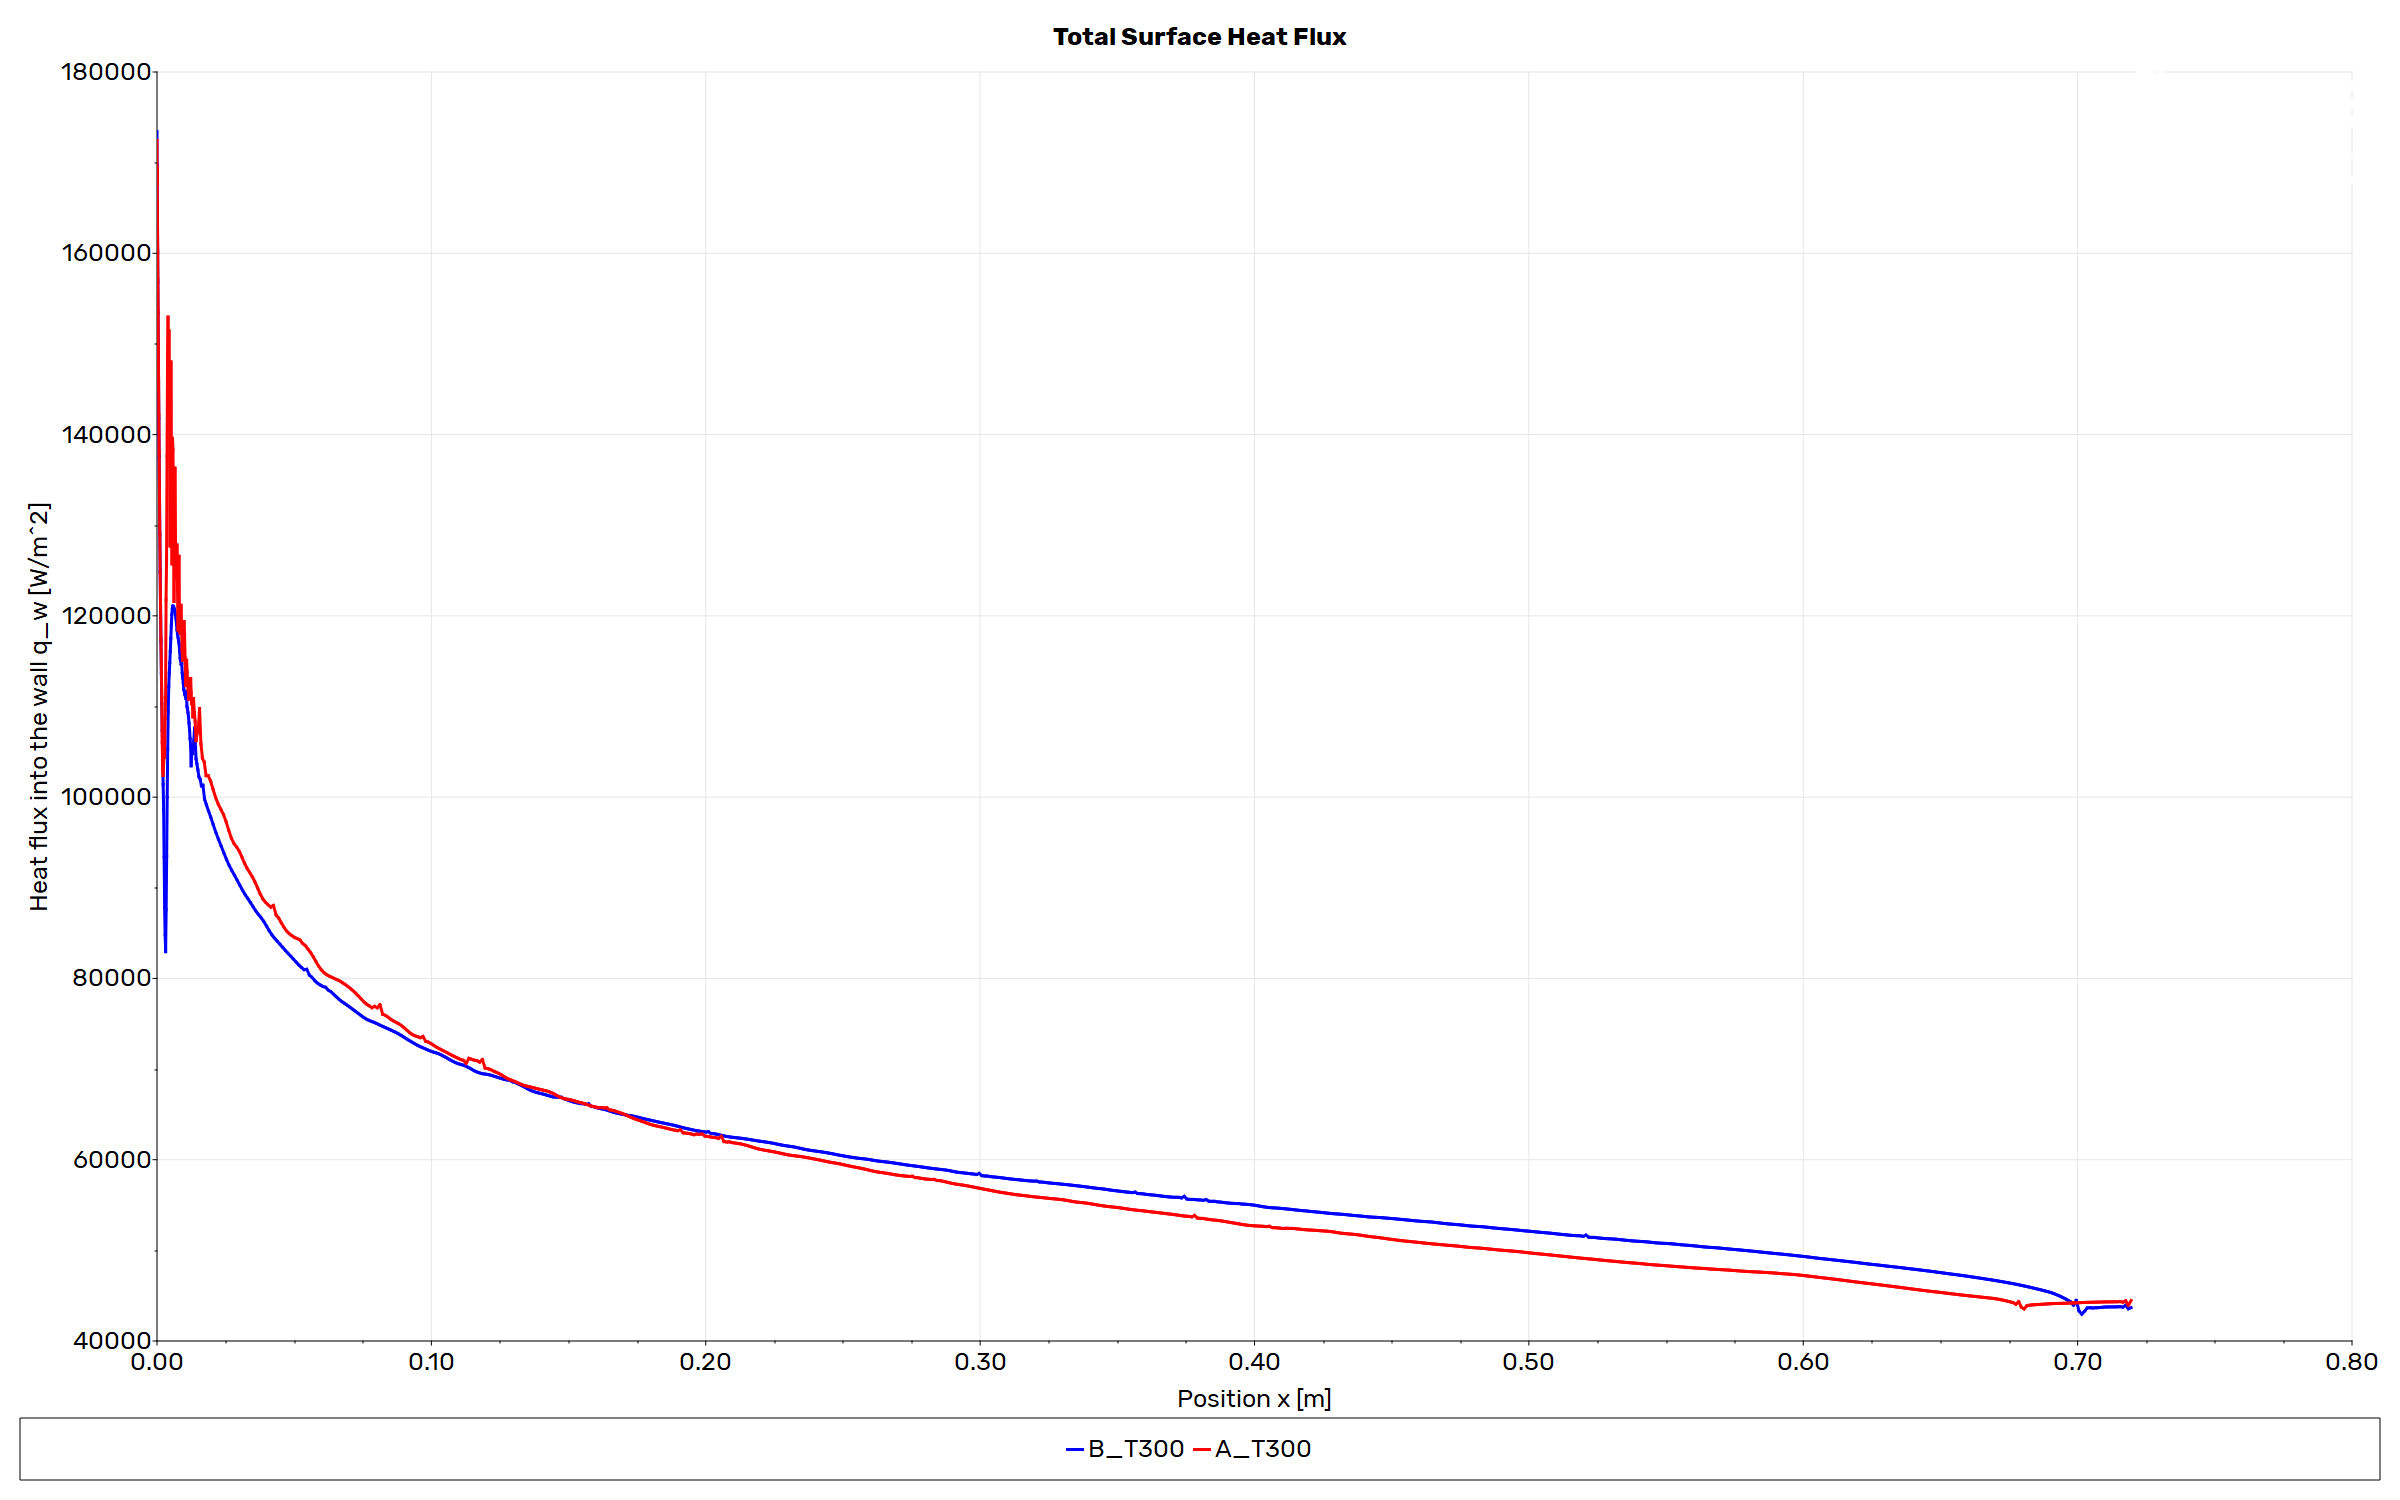
\includegraphics[width=0.9\linewidth]{fluent_qw_AB_T300}
\caption{Heat flux into a wall held at \SI{300}{K} along the nose at burnout, design A (red) and B
(blue), Fluent.}
\label{fig:qw}
\end{figure}

\begin{figure}[H]
\centering
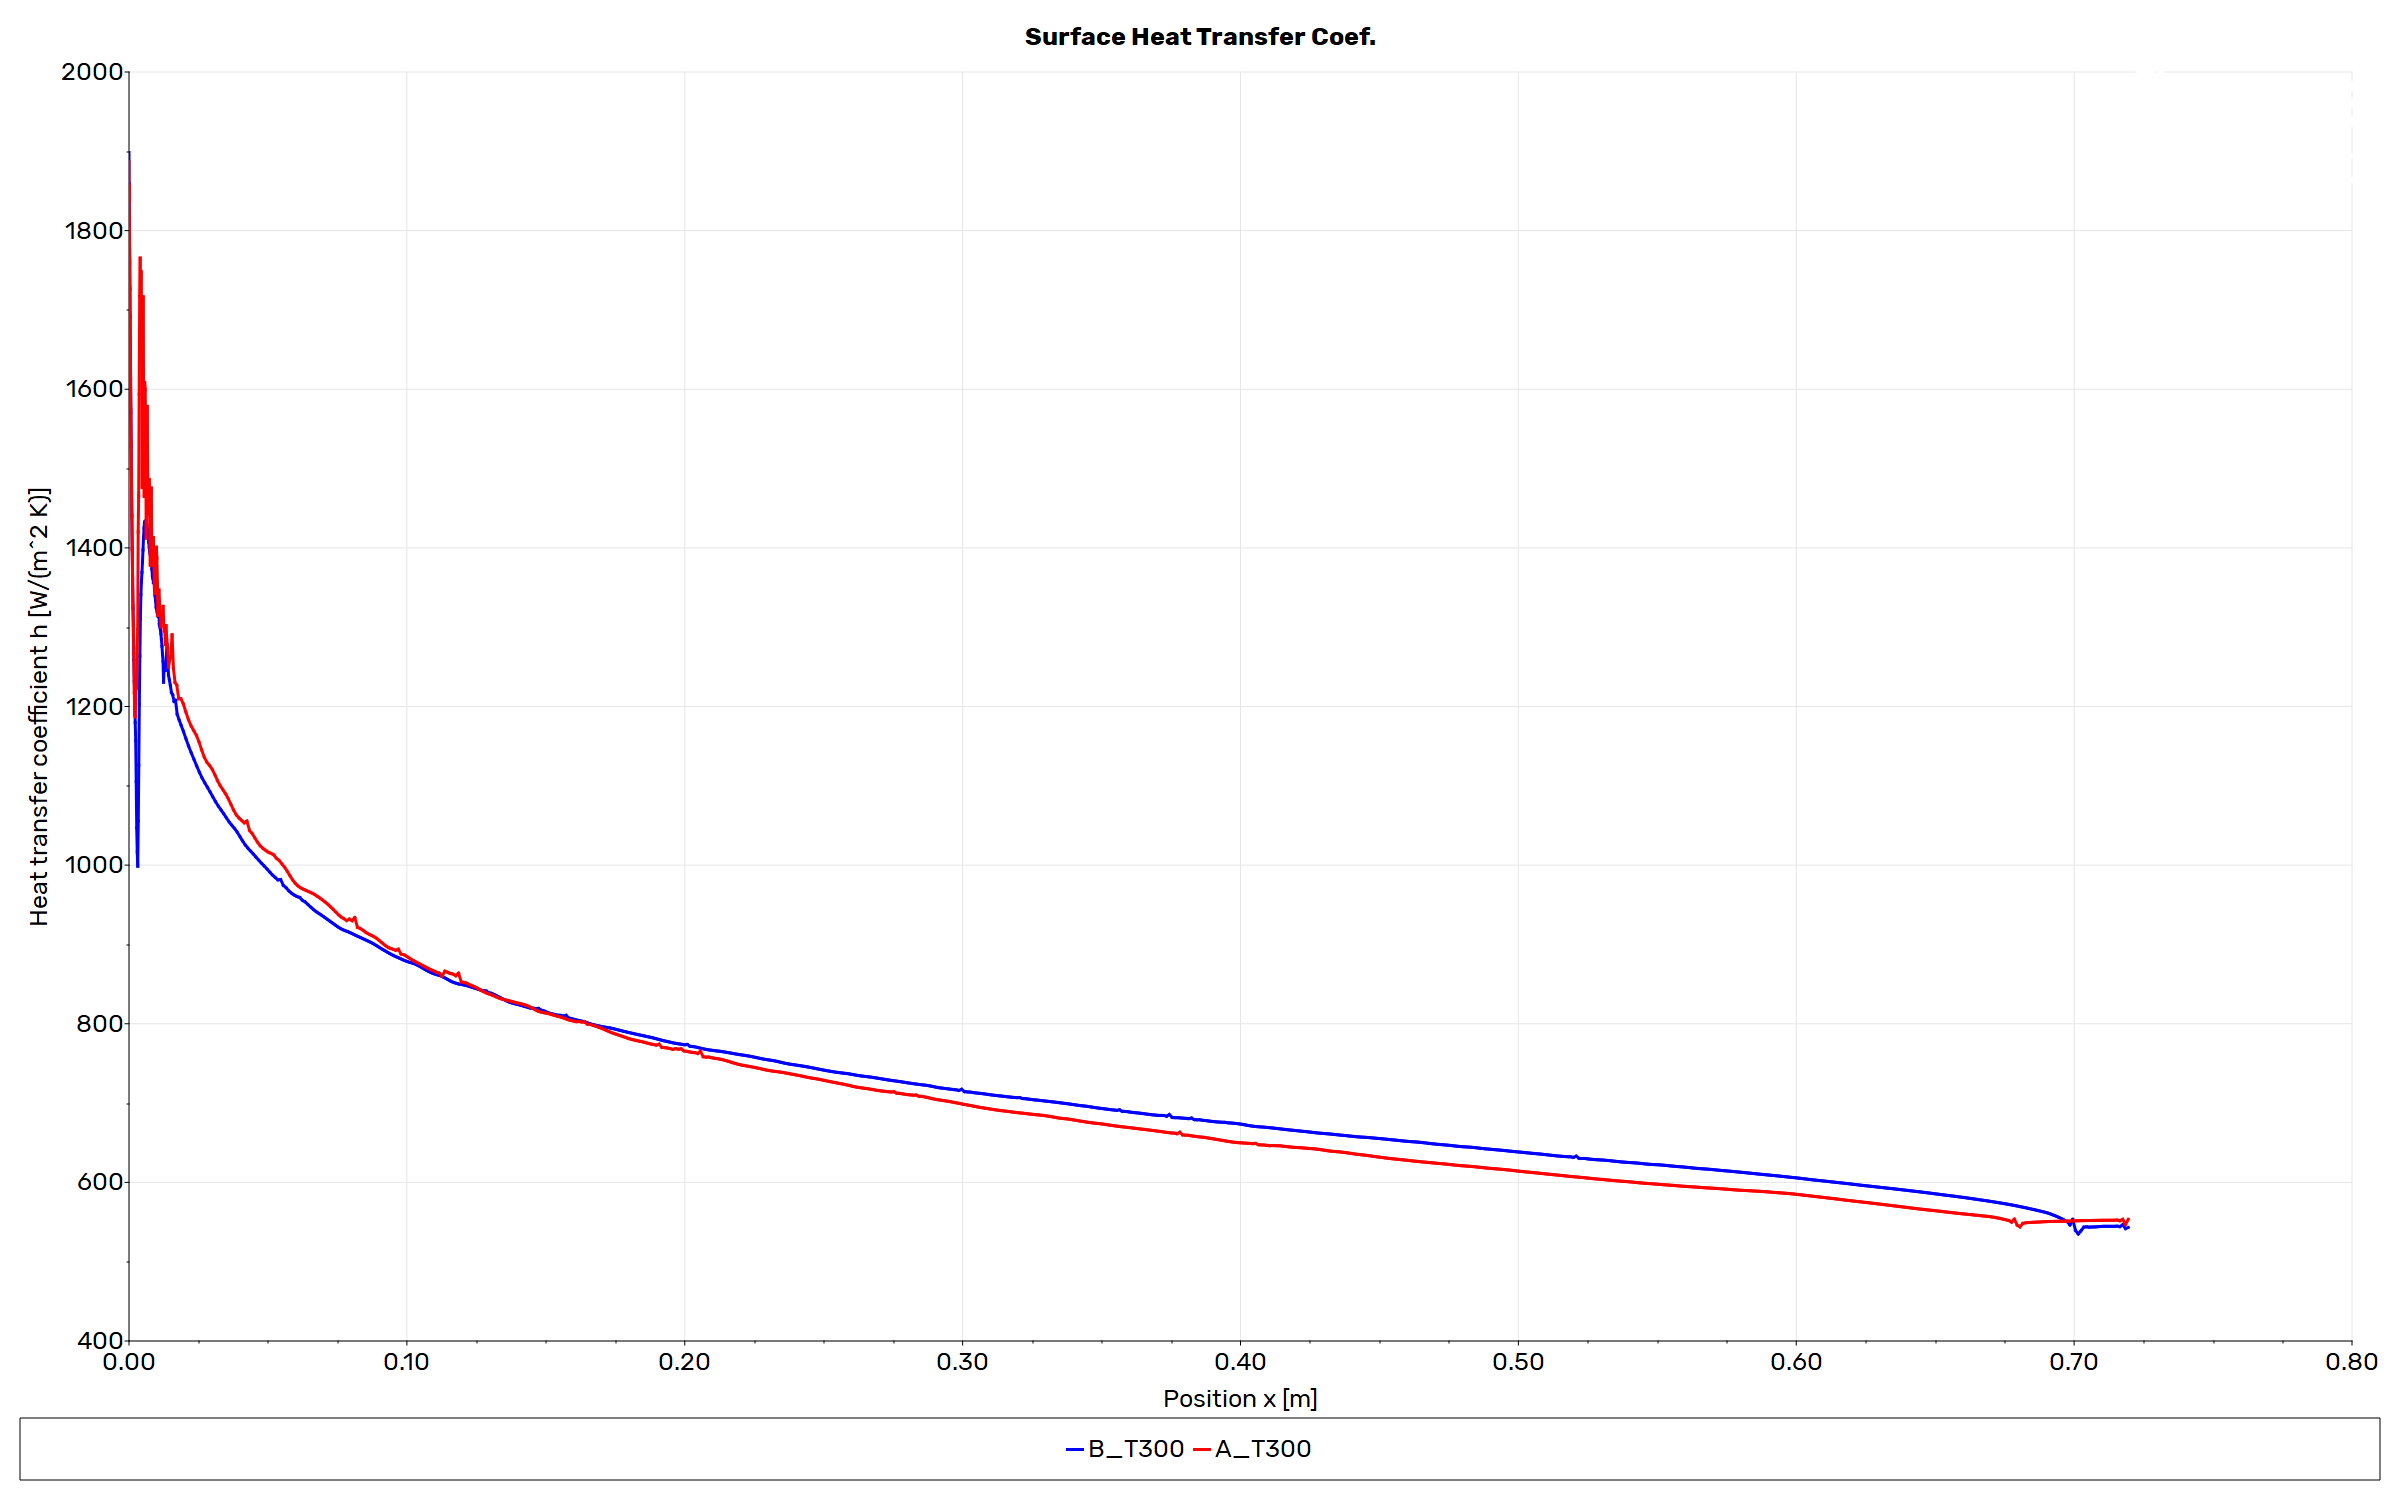
\includegraphics[width=0.9\linewidth]{fluent_h_AB_T300}
\caption{Heat-transfer coefficient $h = q_w / (T_{aw} - \SI{300}{K})$ along the nose at burnout, design A
(red) and B (blue), Fluent. This is the input of the shell model.}
\label{fig:hfluent}
\end{figure}

\begin{table}[H]
\centering
\caption{Heating at burnout from Fluent, nominal day.}
\label{tab:fluentheat}
\small
\begin{tabular}{@{}llcc@{}}
\toprule
 & Unit & Design A & Design B\\
\midrule
Stagnation temperature of the air & K & \val{T0-burnout} & \val{T0-burnout}\\
Wall temperature (adiabatic) at the tip & K & \val{A-Taw0} & \val{B-Taw0}\\
Wall temperature (adiabatic) beyond 50\,mm & K & \val{A-Taw-far-lo}--\val{A-Taw-far-hi} & \val{B-Taw-far-lo}--\val{B-Taw-far-hi}\\
Heat flux at the tip, wall at \SI{300}{K} & kW/m$^2$ & \val{A-qw0} & \val{B-qw0}\\
Heat-transfer coefficient $h$ at the tip & W/(m$^2$K) & \val{A-h0} & \val{B-h0}\\
Heat-transfer coefficient $h$ at the shoulder & W/(m$^2$K) & \val{A-hS} & \val{B-hS}\\
\bottomrule
\end{tabular}
\end{table}

\subsection{Temperature profile along the nose}

Fluent gives the heating at burnout only. To follow the temperatures through the whole flight, the
Python model of report~1 is used, with its heating calibrated on Fluent (Appendix~\ref{app:heatmethod}).
It computes the heat conduction through the \val{shell-t}\,mm CFRP shell at stations from 10\,mm to the
shoulder, heated on the outside. Two simplifications make the shell temperatures slightly high: no heat
is lost on the inside, and over the first 80\,mm the aluminium tip insert under the shell is ignored.

Figure~\ref{fig:thprofile} gives the \textbf{highest temperature reached during the flight} at every point
of the nose, and Figure~\ref{fig:thmap} shows \textbf{when and where} the shell is hot.
\begin{itemize}
\item Both faces are hottest near the tip and cool towards the shoulder, because $h$ falls along the nose.
\item The outer face stays below the DP490 limit everywhere. The inner face is above Req\_10 everywhere.
\item The inner face lags the outer face by about 2\,s, because the heat needs time to cross the CFRP.
Req\_10 is exceeded from about \val{th-A-nominal-req10-t0}\,s to \val{th-A-nominal-req10-t1}\,s on a
nominal day, and from \val{th-A-hot-req10-t0}\,s to \val{th-A-hot-req10-t1}\,s on a hot day.
\end{itemize}

\begin{figure}[H]
\centering
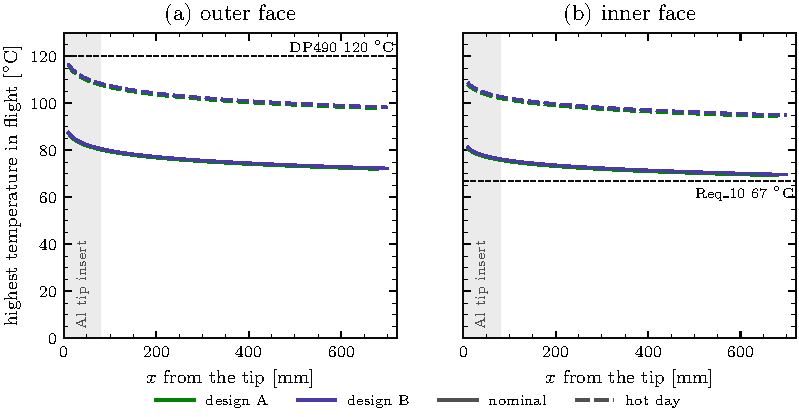
\includegraphics[width=\linewidth]{fig_thermal_profile}
\caption{Highest temperature of the shell during the flight, along the nose: (a) outer face, (b) inner
face. Design A in green, B in purple; solid: nominal day, dashed: hot day. Grey band: the first 80\,mm,
where the aluminium tip insert sits under the shell.}
\label{fig:thprofile}
\end{figure}

\begin{figure}[H]
\centering
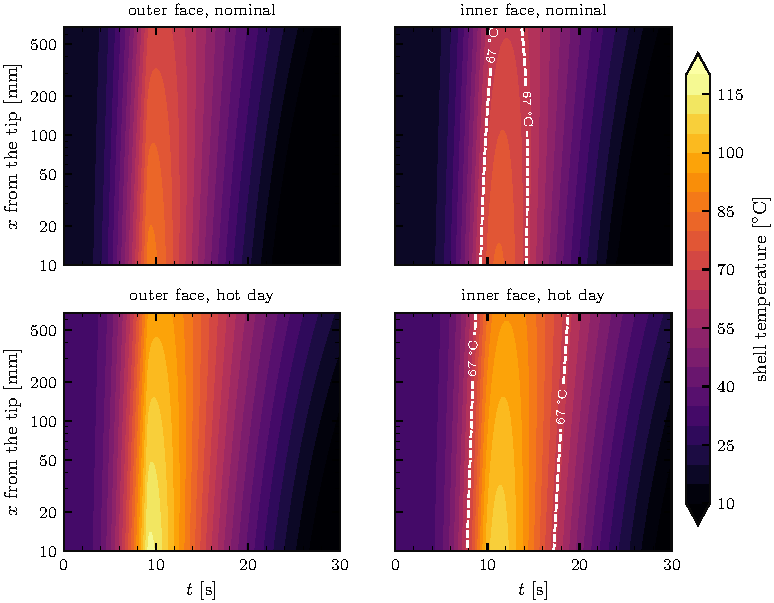
\includegraphics[width=0.8\linewidth]{fig_thermal_map}
\caption{Shell temperature of design A against time and position. Left: outer face; right: inner face.
Top: nominal day; bottom: hot day. White dashed line: \SI{67}{\celsius} (Req\_10) on the inner face. The outer face
stays below \SI{120}{\celsius} (DP490), so it has no line. Design B is the same within \val{th-AB-diff}\,\si{\celsius}.}
\label{fig:thmap}
\end{figure}

\begin{table}[H]
\centering
\caption{Highest shell temperature during the flight at four stations [\si{\celsius}]. \ok: below the limit; \bad: above it.}
\label{tab:thstations}
\small
\begin{tabular}{@{}lccccc@{}}
\toprule
 & \multicolumn{2}{c}{Design A} & \multicolumn{2}{c}{Design B} & \\
\cmidrule(lr){2-3}\cmidrule(lr){4-5}
 & Nominal & Hot day & Nominal & Hot day & Limit\\
\midrule
\grouprow{6}{Outer face}
20\,mm & \val{th-A-nominal-Tout-20} & \val{th-A-hot-Tout-20} & \val{th-B-nominal-Tout-20} & \val{th-B-hot-Tout-20} & 120 (DP490) \ok\\
50\,mm & \val{A-nominal-Tout50} & \val{A-hot-Tout50} & \val{B-nominal-Tout50} & \val{B-hot-Tout50} & 120 (DP490) \ok\\
Mid-length & \val{th-A-nominal-Tout-mid} & \val{th-A-hot-Tout-mid} & \val{th-B-nominal-Tout-mid} & \val{th-B-hot-Tout-mid} & 120 (DP490) \ok\\
Shoulder & \val{th-A-nominal-Tout-shoulder} & \val{th-A-hot-Tout-shoulder} & \val{th-B-nominal-Tout-shoulder} & \val{th-B-hot-Tout-shoulder} & 120 (DP490) \ok\\
\midrule
\grouprow{6}{Inner face}
20\,mm & \val{th-A-nominal-Tin-20} & \val{th-A-hot-Tin-20} & \val{th-B-nominal-Tin-20} & \val{th-B-hot-Tin-20} & 67 (Req\_10) \bad\\
50\,mm & \val{A-nominal-Tin50} & \val{A-hot-Tin50} & \val{B-nominal-Tin50} & \val{B-hot-Tin50} & 67 (Req\_10) \bad\\
Mid-length & \val{th-A-nominal-Tin-mid} & \val{th-A-hot-Tin-mid} & \val{th-B-nominal-Tin-mid} & \val{th-B-hot-Tin-mid} & 67 (Req\_10) \bad\\
Shoulder & \val{th-A-nominal-Tin-shoulder} & \val{th-A-hot-Tin-shoulder} & \val{th-B-nominal-Tin-shoulder} & \val{th-B-hot-Tin-shoulder} & 67 (Req\_10) \bad\\
\bottomrule
\end{tabular}
\end{table}

\subsection{Temperatures during the flight}

Figure~\ref{fig:temps} follows the parts that matter most for ST through the flight: the aluminium tip
insert, the shell at 50\,mm (inside the region of the insert) and the air inside the nose. The peaks of
the tip insert and the inside air are in Table~\ref{tab:heat}, those of the shell in
Table~\ref{tab:thstations}.
\begin{itemize}
\item The outer face of the shell peaks just after burnout (9.6\,s), the inner face 2\,s later.
\item The tip insert, with its larger heat capacity, peaks later, at 12--13\,s, and cools slowly.
\item The tip insert of design B gets \SI{20}{\percent} less heat than A's (its front is thinner, so there
is less surface in the first 80\,mm) and stays 5--6\,\si{\celsius} cooler.
\item The air inside follows the inner face of the shell (upper bound). Whether Req\_10 applies to the air or
to the inner wall is still open with SE.
\end{itemize}

\begin{figure}[H]
\centering
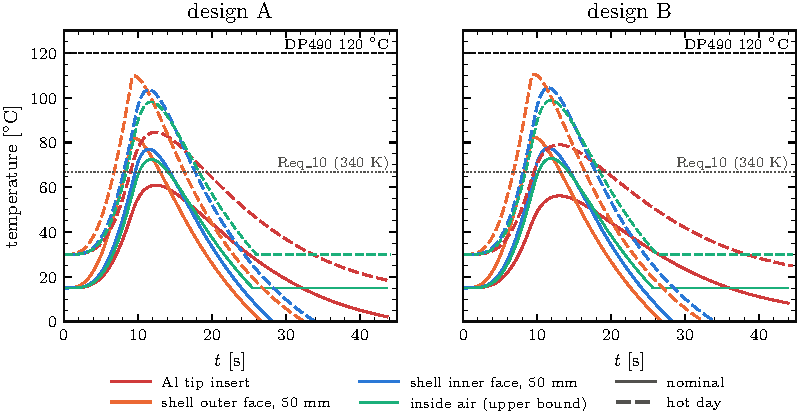
\includegraphics[width=\linewidth]{fig_temperatures}
\caption{Temperatures during the flight, design A (a) and B (b): aluminium tip insert, CFRP shell at
50\,mm (outer and inner face) and the inside air (upper bound). Solid: nominal day; dashed: hot day.}
\label{fig:temps}
\end{figure}

\begin{table}[H]
\centering
\caption{Highest stagnation, tip-insert and inside-air temperatures during the flight (the shell is
in Table~\ref{tab:thstations}). \bad: above the limit. Tip insert: Al\,6082, \val{tip-mass}\,g over the first
\val{tip-length}\,mm.}
\label{tab:heat}
\small
\begin{tabular}{@{}llccccc@{}}
\toprule
 & & \multicolumn{2}{c}{Design A} & \multicolumn{2}{c}{Design B} & \\
\cmidrule(lr){3-4}\cmidrule(lr){5-6}
 & Unit & Nominal & Hot day & Nominal & Hot day & Limit\\
\midrule
Stagnation temperature of the air & \si{\celsius} & \val{A-nominal-T0} & \val{A-hot-T0} & \val{B-nominal-T0} & \val{B-hot-T0} & \\
Aluminium tip insert & \si{\celsius} & \val{A-nominal-Ttip} & \val{A-hot-Ttip} & \val{B-nominal-Ttip} & \val{B-hot-Ttip} & \\
Inside air, upper bound & \si{\celsius} & \val{A-nominal-Tair} & \val{A-hot-Tair} & \val{B-nominal-Tair} & \val{B-hot-Tair} & 67 (Req\_10) \bad\\
\bottomrule
\end{tabular}
\end{table}

